%%%%%%%%%%%%%%%%%%%%%%%%%%%%%%%%%%%%%%%%%%%%%%%%%%%%%%%%%%%%%%%%%%%%%%%%%%%%%%%%
%% Plantilla de memoria en LaTeX para la ETSIT - Universidad Rey Juan Carlos
%%
%% Por Gregorio Robles <grex arroba gsyc.urjc.es>
%%     Grupo de Sistemas y Comunicaciones
%%     Escuela Técnica Superior de Ingenieros de Telecomunicación
%%     Universidad Rey Juan Carlos
%% (muchas ideas tomadas de Internet, colegas del GSyC, antiguos alumnos...
%%  etc. Muchas gracias a todos)
%%
%% La última versión de esta plantilla está siempre disponible en:
%%     https://github.com/gregoriorobles/plantilla-memoria
%%
%% Para obtener PDF, ejecuta en la shell:
%%   make
%% (las imágenes deben ir en PNG o JPG)

%%%%%%%%%%%%%%%%%%%%%%%%%%%%%%%%%%%%%%%%%%%%%%%%%%%%%%%%%%%%%%%%%%%%%%%%%%%%%%%%

\documentclass[a4paper, 12pt]{book}
%\usepackage[T1]{fontenc}

\usepackage[a4paper, left=2.5cm, right=2.5cm, top=3cm, bottom=3cm]{geometry}
\usepackage{times}
\usepackage[utf8]{inputenc}
\usepackage[spanish]{babel} % Comenta esta línea si tu memoria es en inglés
\usepackage{url}
%\usepackage[dvipdfm]{graphicx}
\usepackage{graphicx}
\usepackage{float}  %% H para posicionar figuras
\usepackage[nottoc, notlot, notlof, notindex]{tocbibind} %% Opciones de índice
\usepackage{latexsym}  %% Logo LaTeX

\title{Memoria del Proyecto}
\author{Vicente Giménez García}

\renewcommand{\baselinestretch}{1.5}  %% Interlineado

\begin{document}

\renewcommand{\refname}{Bibliografía}  %% Renombrando
\renewcommand{\appendixname}{Apéndice}

%%%%%%%%%%%%%%%%%%%%%%%%%%%%%%%%%%%%%%%%%%%%%%%%%%%%%%%%%%%%%%%%%%%%%%%%%%%%%%%%
% PORTADA

\begin{titlepage}
\begin{center}

\includegraphics[scale=0.8]{img/URJ_logo_Color_POS.png}

\vspace{1.75cm}

\Large
GRADO EN INGENIERÍA EN TECNOLOGÍAS DE TELECOMUNICACIÓN

\vspace{0.4cm}

\large
Curso Académico 2020/2021

\vspace{0.8cm}

Trabajo Fin de Grado

\vspace{2.5cm}

\LARGE
[TODO] TÍTULO DEL TRABAJO EN MAYÚSCULAS

\vspace{4cm}

\large
Autor : Vicente Giménez García \\
Tutor : Pedro de las Heras Quirós
\end{center}
\end{titlepage}

\newpage
\mbox{}
\thispagestyle{empty} % para que no se numere esta pagina


%%%%%%%%%%%%%%%%%%%%%%%%%%%%%%%%%%%%%%%%%%%%%%%%%%%%%%%%%%%%%%%%%%%%%%%%%%%%%%%%
%%%% Para firmar
\clearpage
\pagenumbering{gobble}
\chapter*{}

\vspace{-4cm}
\begin{center}
\LARGE
\textbf{Trabajo Fin de Grado}

\vspace{1cm}
\large
[TODO] Título del Trabajo con Letras Capitales para Sustantivos y Adjetivos

\vspace{1cm}
\large
\textbf{Autor :} Vicente Giménez García \\
\textbf{Tutor :} Pedro de las Heras Quirós

\end{center}

\vspace{1cm}
La defensa del presente Proyecto Fin de Carrera se realizó el día \qquad$\;\,$ de \qquad\qquad\qquad\qquad \newline de 2021, siendo calificada por el siguiente tribunal:


\vspace{0.5cm}
\textbf{Presidente:}

\vspace{1.2cm}
\textbf{Secretario:}

\vspace{1.2cm}
\textbf{Vocal:}


\vspace{1.2cm}
y habiendo obtenido la siguiente calificación:

\vspace{1cm}
\textbf{Calificación:}


\vspace{1cm}
\begin{flushright}
Fuenlabrada, a \qquad$\;\,$ de \qquad\qquad\qquad\qquad de 202X
\end{flushright}

%%%%%%%%%%%%%%%%%%%%%%%%%%%%%%%%%%%%%%%%%%%%%%%%%%%%%%%%%%%%%%%%%%%%%%%%%%%%%%%%
%%%% Dedicatoria

\chapter*{}
\pagenumbering{Roman} % para comenzar la numeracion de paginas en numeros romanos
\begin{flushright}
\textit{[TODO] Dedicado a \\
mi familia / mi abuelo / mi abuela}
\end{flushright}

%%%%%%%%%%%%%%%%%%%%%%%%%%%%%%%%%%%%%%%%%%%%%%%%%%%%%%%%%%%%%%%%%%%%%%%%%%%%%%%%
%%%% Agradecimientos

\chapter*{Agradecimientos}
%\addcontentsline{toc}{chapter}{Agradecimientos} % si queremos que aparezca en el índice
\markboth{AGRADECIMIENTOS}{AGRADECIMIENTOS} % encabezado

[TODO]

%%%%%%%%%%%%%%%%%%%%%%%%%%%%%%%%%%%%%%%%%%%%%%%%%%%%%%%%%%%%%%%%%%%%%%%%%%%%%%%%
%%%% Resumen

\chapter*{Resumen}
%\addcontentsline{toc}{chapter}{Resumen} % si queremos que aparezca en el índice
\markboth{RESUMEN}{RESUMEN} % encabezado

Una de las dificultades a las que se enfrentan los alumnos en período de prácticas empresariales o recién egresados de la universidad
es el desconocimiento de qué salario podría considerarse justo para un determinado puesto ante una oferta de trabajo.

A esta dificultad se añade el hecho de que muichos trabajadores consideran hablar de su sueldo un tema tabú,
lo que complica a aquellos alumnos que buscan trabajo la tarea de recabar información acerca de qué rango salarial es el adecuado para una determinada actividad.

Además, concretamente en el ámbito de las tecnologías de la información y la comunicación, el gran abanico de sectores, profesiones, técnicas, lenguajes, etcétera,
hace que resulte realmente complejo para una persona con poca experiencia evaluar si una oferta de trabajo es interesante desde un punto de vista económico.

Con el objetivo de facilitar a los alumnos esta tarea de entendimiento del mercado, este proyecto pretende plantear una solución sencilla y eficaz en forma de aplicación
web que permite buscar y compartir información laboral de primera mano a través de las experiencias laborales de los usuarios que participan en la plataforma.

Esta aplicación enfatiza en el intercambio de información laboral entre dos usuarios como fuente información, permitiendo en todos los casos que estos compartan únicamente los datos que deseen mostrar acerca de una experiencia laboral propia,
incluida su identidad en caso de que prefieran ofrecer sus referencias de forma anónima.

Este proyecto se compone de un servidor que expone su funcionalidad a través de un API REST, desarrollado con la tecnología Spring Boot y una aplicación de navagdor en el lado del cliente desarrollada en React que consume los recursos expuestos en dicha API.
Todo el sistema es accesible a través de autenticación de los usuarios en la plataforma de Github, lo que permite a la mayoría de los alumnos de grados relacionados con las TIC poder hacer uso de la aplicación sin tener que hacer un registro adicional.

%%%%%%%%%%%%%%%%%%%%%%%%%%%%%%%%%%%%%%%%%%%%%%%%%%%%%%%%%%%%%%%%%%%%%%%%%%%%%%%%
%%%%%%%%%%%%%%%%%%%%%%%%%%%%%%%%%%%%%%%%%%%%%%%%%%%%%%%%%%%%%%%%%%%%%%%%%%%%%%%%
% ÍNDICES %
%%%%%%%%%%%%%%%%%%%%%%%%%%%%%%%%%%%%%%%%%%%%%%%%%%%%%%%%%%%%%%%%%%%%%%%%%%%%%%%%.

%%%% Índice de contenidos
\tableofcontents
%%%% Índice de figuras
\cleardoublepage
%\addcontentsline{toc}{chapter}{Lista de figuras} % para que aparezca en el indice de contenidos
\listoffigures % indice de figuras
%%%% Índice de tablas
%\cleardoublepage
%\addcontentsline{toc}{chapter}{Lista de tablas} % para que aparezca en el indice de contenidos
%\listoftables % indice de tablas


%%%%%%%%%%%%%%%%%%%%%%%%%%%%%%%%%%%%%%%%%%%%%%%%%%%%%%%%%%%%%%%%%%%%%%%%%%%%%%%%
%%%%%%%%%%%%%%%%%%%%%%%%%%%%%%%%%%%%%%%%%%%%%%%%%%%%%%%%%%%%%%%%%%%%%%%%%%%%%%%%
% INTRODUCCIÓN %
%%%%%%%%%%%%%%%%%%%%%%%%%%%%%%%%%%%%%%%%%%%%%%%%%%%%%%%%%%%%%%%%%%%%%%%%%%%%%%%%

\cleardoublepage
\chapter{Introducción}
\label{sec:intro} % etiqueta para poder referenciar luego en el texto con ~\ref{sec:intro}
\pagenumbering{arabic} % para empezar la numeración de página con números

Este Trabajo fin de Grado consiste en una aplicación web desarrollada en una arquitectura cliente-servidor que tiene el próposito de permitir a los usuarios crear, modificar y eliminar sus experiencias laborales con un nivel de privacidad establecido por el propio usuario
de forma que sean accesibles mediante una búsqueda por el resto de los usuarios, que pueden solicitar información privada acerca de estas a cambio de ofrecer la suya propia.
En esta arquitectura, el cliente es una aplicación JavaScript ejecutable en el navegador,
y el servidor es un servidor de aplicaciones Java EE cuyos recursos son accesibles por el cliente a través de un API REST. Además, la aplicación utiliza GitHub como proveedor de autenticación para los usuarios.
A continuación se procederá a describir tanto cada una de las partes de la aplicación como las tecnologías utilizadas y las herramientas empleadas para su desarrollo.

\section{Definición de experiencia laboral}
\label{sec:intro_workexperiencedefinition}
En el contexto de este Trabajo Fin de Grado, se considerará una experiencia laboral de un usuario al conjunto de datos formados por:

\begin{itemize}
  \item La empresa donde transcurrió la experiencia laboral.
  \item El puesto que se desempeñó dentro de la empresa.
  \item El conjunto de tecnologías de las que el usuario hizo uso durante el ejercicio de su actividad.
  \item El periodo durante el que se ejerció la actividad en la empresa, con fecha de inicio y fecha de fin en el caso de experiencias pasadas.
  \item El salario bruto anual representativo que percibió el usuario durante el periodo laboral.
\end{itemize}

\section{Privacidad}
\label{sec:intro_privacity}
Para cada una de las experiencias que un usuario agregue al sistema, este podrá decidir todo momento la visibilidad que tendrá cada uno de los campos de la definición de experiencia laboral para el resto de usuarios, siendo posible que un campo sea público, lo que lo hará visible para la totalidad de los usuarios, o privado, en cuyo caso solo será visible para aquellos usuarios que mediante  una solicitud de información hayan obtenido permiso para visualizar dicho campo.

Adicionalmente, los usuarios podrán elegir dentro de sus experiencias, cuales de ellas serán vinculadas a su perfil. Aquellas que no sean vinculadas aparecerán vinculadas a un usuario anónimo en las búsquedas que hagan el resto de usuarios, siendo imposible reconocer a quién pertenecen.

\section{Solicitud de información a otros usuarios}
\label{sec:intro_inforequest}
Dada una experiencia laboral determinada, en la que uno o varios de los campos hayan sido declarados como privados por su poseedor, es posible para otros usuarios solicitar revelar estos campos.
Para esto el usuario interesado envía una solicitud de información en la que indica cuales de estos campos quiere que le sean revelados, y opcionalmente, ofrece revelar campos privados de alguna de sus experiencias a cambio al usuario receptor de la solicitud.
En este momento se establece una negociación entre ambos usuarios, en el que cada uno de ellos, por turnos, puede modificar lo que ofrece y solicita revelar. Esta negociación finalizada cuando el usuario al que corresponde realizar el siguiente paso de la negociación acepta el intercambio de datos, o en el momento en el que uno de ambos usuarios deniega la solicitud.


\section{Servidor de aplicaciones}
\label{sec:intro_applicationserver}

Es la pieza de software que no se ejecuta en el navegador si no que es invocada desde este vía conexión HTTP.
Su cometido en la aplicación es el de exponer recursos que ofrecen la información de los usuarios, es decir, sus experiencias laborales y solicitudes de manera controlada basada en la identidad de los usuarios.
Para ello antes de ofrecer información al lado cliente comprueba la identidad del usuario que la solicita para aplicarle las reglas de visibilidad y presentar únicamente la información que,
o bien es pública, o bien pertenece al solicitante, o bien tanto el solicitante como el propietario han accedido a compartir. Abajo se describirán los puntos principales relacionados con el servidor de aplicaciones.

\subsection{Lenguaje y plataforma}
\label{subsec:intro_applicationserver_languageandplatform}

El lenguaje elegido para el desarrollo del servidor es Java. Java es un lenguaje de programación orientada objetos desarrollado por la compañía Sun Microsystems.
Una de sus particularidades más importantes es la de poder ejecutarse en la máquina virtual de Java (JVM) que puede ser instalada en la gran mayoría de sistemas operativos,
lo que proporciona a este lenguaje gran portabilidad entre distintas plataformas. La versión concreta de Java que se utilizó para el desarrollo fue la 11, que entre otras características da Java soporte para la programación funcional.

El framework Java utilizado para la creación del servidor fue Spring, un framework Open Source que facilita el desarrollo de aplicaciones Java Enterprise Edition, que es a su vez una plataforma, parte de la plataforma Java que permite el desarrollo de aplicaciones servidor.
Spring Framework provee una serie de características y librerías que ayudan al programador a centrarse en el desarrollo de la lógica que quiere implementar en su aplicación, abstrayéndose de conceptos de infraestructura que complican el desarrollo de servidores.
 Para esta aplicación se utilizó concretamente la tecnología Spring Boot que además reduce la cantidad de configuración necesaria para funcionamiento de una aplicación Spring.

\subsection{Comunicación con el cliente}
\label{subsec:intro_applicationserver_communicationwithclient}

Para permitir a la parte cliente del navegador acceder la información laboral que reside en el servidor, la aplicación servidor expone un API REST.
Un API REST es una interfaz accesible de forma remota vía protocolo HTTP donde la información se representa en forma de recurso, siendo estos recursos identificadores de los conceptos y entidades que alberga el servidor, que en el caso de este Trabajo Fin de Grado son las experiencias laborales y las solicitudes de información.
En un API REST estos recursos son operables utilizando los propios métodos HTTP, a los que el estilo REST provee de semántica, interpretándose los verbos HTTP como operaciones de escritura, lectura, borrado y modificación. De esta forma un cliente web puede en este caso crear, borrar, leer y modificar experiencias laborales y solicitudes dentro del servidor enviando mensajes HTTP.

\subsection{Base de datos}
\label{subsec:intro_applicationserver_database}

Para almacenar las experiencias laborales de los usuarios y solicitudes, el servidor hace uso de una base de datos relacional (SQL), concretamente H2, que es un motor de bases de datos Open Source cuyas características principales son estar implementado en Java,
lo que simplifica en muchos casos la integración con aplicaciones Java, y el poder levantarse en memoria o en modo embebido, de forma que sus datos se almacenan en ficheros, lo que facilita la base de desarrollo, evitando al programador tener que instalar y configurar una base de datos completa.
El dialecto SQL que utiliza H2 es altamente compatible con el resto de dialectos de SQL, lo que a futuro permite hacer uso de otro distribuidor distinto de base de datos sin realizar grandes modificaciones.

Como librería para realizar operaciones de base de datos desde el servidor se ha hecho uso de MyBatis, una herramienta de persistencia de Java que permite definir sentencias SQL en archivos XML que pueden ser invocadas desde el código y que integra fácilmente con Spring Framework.

La herramienta para definir la estructura de la base de datos es Flyway, una tecnología que permite llevar un versionado de la base de datos mediante una lista de scripts SQL, uno por versión. Estos scripts se ejecutan secuencialmente, por lo que cada script debe escribirse como una modificación del estado de la estructura de base de datos que dejó el script anterior.
De esta manera Flyway es capaz de llevar un registro de que modificaciones se hicieron en anteriores desarrollos sobre el proyecto, para ejecutar solo los nuevos scripts, es decir, los últimos cambios, no teniendo que generar una estructura nueva en cada modificación, lo que facilita la modificación de la base de datos una vez la aplicación está en producción,
sin la pérdida de datos que supondría eliminar toda la estructura SQL y volverla a crear en cada modificación.


\section{Aplicación web}
\label{sec:intro_webapplication}

Es la aplicación que se ejecuta en el navegador web del usuario. Su función es la de ofrecer una interfaz amigable e intuitiva al usuario para permitirle operar sobre sus recursos en el servidor y realizar consultas de datos.
En el caso concreto de este Trabajo Fin de Grado, la aplicación web ofrece una interfaz para que el usuario pueda crear, modificar e eliminar sus experiencias laborales, realizar búsquedas de experiencias laborales mediante filtros
y crear solicitudes de datos confidenciales a otros usuarios desde su navegador, mediante una interfaz gráfica.

\subsection{Lenguaje y librerías}
\label{subsec:intro_webapplication_languageandlibraries}

El lenguaje utilizado para desarrollar la lógica en esta parte fue JavaScript. Este es un lenguaje interpretado orientado a objetos, que se ejecuta en los navegadores y permite modificar el documento HTML que visualiza el usuario, solicitar datos remotos a un servidor y almacenar datos en el propio navegador entre otras funciones.

La librería utilizada para el desarrollo de la aplicación fue React, una librería que facilita el desarrollo de aplicaciones JavaScript de una sola página, cuya característica principal es la facilidad que aporta a la hora de desarrollar componentes web, es decir,
componentes reutilizables en la aplicación, que se pueden invocar múltiples veces en el código mediante una etiqueta y atributos que actúan como entrada de información en el componente, y que tienen su propia estructura interna, comportamiento y estilo.
Para esto React hace uso de archivos JavaScript con una extensión específica, JSX, que permiten referenciar HTML directamente desde el código JavaScript como si se tratara de un tipo de dato adicional a los que el JavaScript nativo soporta.
Debido al uso de esta librería, la presencia de archivos HTML en la aplicación web es mínima, limitándose a un único archivo prácticamente vacío cuya función es referenciar los recursos necesarios para la ejecución de la aplicación.


\subsection{Estilo}
\label{subsec:intro_webapplication_style}

Para agregar estilos a la interfaz gráfica y hacer la aplicación visualmente más atractiva se ha hecho uso de la librería Bootstrap. Bootstrap provee una serie de estilos CSS predefinidos y fácilmente utilizables sobre los elementos HTML de la aplicación en forma de clases HTML.

\section{Autenticación}
\label{sec:intro_authentication}

Con el objetivo de facilitar a los usuarios el ingreso en la aplicación, esta se ha integrado con la plataforma GitHub, haciendo uso de ella como proveedora de autenticación e identidad. De esta manera, los usuarios que ya están registrados en GitHub, como suele ser el caso de los alumnos de carreras relacionadas con las TIC, pueden utilizar sus credenciales de GitHub para acceder a la aplicación. Estas credenciales se envían directamente a GitHub, por lo que no pasan directamente por la aplicación de este Trabajo Fin de Grado, de forma que en ningún momento se pone en riesgo la privacidad del usuario.

Para lograr esto se ha hecho uso del módulo Spring Social, que facilita la comunicación con GitHub vía el estándar OAuth2, una forma de integrar aplicaciones con plataformas que ofrecen parte de los datos de sus usuarios sin vulnerar su privacidad, extendiendo la sesión de estos usuarios a aplicaciones de terceros.


\section{Herramientas}
\label{sec:intro_tools}
A continuación se exponen brevemente algunas de las principales herramientas que se utilizaron para el desarrollo de la aplicación.

\subsection{IntelliJ IDEA}
\label{subsec:intro_tools_intellij}
IntelliJ IDEA es un entorno de desarrollo integrado desarrollado por la compañía JetBrains. Tiene soporte para el lengauje Java, facilita las tareas de escritura del código, permite ejecutar y depurar aplicaciones y pruebas, integra con varias herramientas de gestión de dependencias y control de versiones, entre otras características. Se eligió este IDE para hacer el desarrollo del servidor de aplicaciones.

\subsection{Visual Studio Code}
\label{subsec:intro_tools_vsc}
Visual Studio Code es un editor de código fuente con gran soporte para JavaScript. Permite ejecutar y depurar aplicaciones y pruebas, integra con gestores de dependencias y control de versiones. Se eligió este editor para el desarrollo de la aplicación web en React.

\subsection{Maven}
\label{subsec:intro_tools_maven}
Maven es una herramienta de gestión de proyectos de software desarrollada por Apache Software Foundation. Permite de forma declarativa gestionar todas las dependencias de un proyecto Java, es decir, referenciar los módulos que contienen las librerías sobre las que se construye el proyecto para poder descargarlos automáticamente del repositorio central de Maven
durante la construcción de la aplicación. También permite la ejecución de plugins que facilitan tareas de desarrollo como construcción, ejecución de pruebas, empaquetado, instalación, etcétera. Se utilizó para la gestión de dependecias del servidor de aplicaciones.

\subsection{NPM}
\label{subsec:intro_tools_npm}
NPM es el sistema de gestión de paquetes para el lenguaje JavaScript. De forma similar a Maven permite gestionar las dependencias de una aplicación web JavaScript declarándolas en un fichero y automatizando de esta forma su descarga. Se utilizó para la gestión de dependencias de la aplicación web.


\subsection{Git}
\label{subsec:intro_tools_git}
Git es un sistema de control de versiones distribuido y de código abierto. Permite mantener un histórico de los cambios del proyecto de forma remota (en este caso en Github) y una copia de estos de forma local. Además permite mantener distintas ramas de desarollo en paralelo, esta característica facilita el desarollo de distintas funcionalidades del software en paralelo, ya sea por uno o varios desarrolladores, siendo posible mezclar estas distintas ramas después con la versión final, gestionando mediante el sistema Git las diferencias y conflictos entre los cambios en el código.

\section{Estructura de la memoria}
\label{sec:intro_memorystructure}
[TODO]


%%%%%%%%%%%%%%%%%%%%%%%%%%%%%%%%%%%%%%%%%%%%%%%%%%%%%%%%%%%%%%%%%%%%%%%%%%%%%%%%
%%%%%%%%%%%%%%%%%%%%%%%%%%%%%%%%%%%%%%%%%%%%%%%%%%%%%%%%%%%%%%%%%%%%%%%%%%%%%%%%
% OBJETIVOS %
%%%%%%%%%%%%%%%%%%%%%%%%%%%%%%%%%%%%%%%%%%%%%%%%%%%%%%%%%%%%%%%%%%%%%%%%%%%%%%%%

\cleardoublepage % empezamos en página impar
\chapter{Objetivos} % título del capítulo (se muestra)
\label{chap:targets} % identificador del capítulo (no se muestra, es para poder referenciarlo)

\section{Objetivo general} % título de sección (se muestra)
\label{sec:targets_generaltarget} % identificador de sección (no se muestra, es para poder referenciarla)

El objetivo de este Trabajo Fin de Grado es desarrollar una aplicación que permita a estudiantes y trabajadores del sector de las tecnologías de la información y la comunicación evaluar cual es el rango salarial justo para una determinada profesión u oferta de trabajo teniendo en cuenta la empresa donde se realizará la labor, el cargo y las tecnologías relacionadas con el puesto.


\section{Objetivos específicos}
\label{sec:target_specifictargets}

Los objetivos específicos de este Trabajo Fin de Grado son:

\begin{enumerate}
  \item Proporcionar a los usuarios del sector TIC un método para ingresar fácilmente en la aplicación sin necesidad de registrarse, mediante un proveedor de autenticación externo.
  \item Permitir a los usuarios añadir, modificar y eliminar sus experiencias laborales en el sistema a través de la aplicación.
  \item Dar opción a los usuarios para que estas experiencias laborales no se vinculen con su perfil, de manera que sean visibles a otros usuarios sin conocer la identidad de aquel al que pertenecen.
  \item Permitir a los usuarios declarar parte o todos los datos relacionados con una de sus experiencias laborales como privados de forma que solo sean visibles para otros usuarios mediante un acuerdo con el poseedor.
  \item Proporcionar a los usuarios un mecanismo de búsqueda de experiencias laborales de otros usuarios.
  \item Permitir filtrar estas búsquedas por puesto, empresa, tecnologías, salario mínimo y máximo y fecha de inicio mínima y máxima.
  \item Dar opción a los usuarios de solicitar información privada de una experiencia ajena mediante el envío de un solcitud a su propietario, pudiendo ofrecer el solicitante datos privados de alguna de sus propias experiencias a cambio.
  \item Ofrecer un mecanismo para que los usuarios puedan renegociar por turnos que datos mostrarán y solicitan sobre una determinada solicitud.
  \item Ofrecer un mecanismo para poder aceptar o denegar solicitudes de datos privados.
  \item Permitir ver a los usuarios el histórico de los estados por los que ha pasado la negociación de una solcitud en vuelo o finalizada.
  \item En caso de que una solicitud de datos sea aceptada, permitir a los usuarios visualizar los datos privados ahora visibles como resultado de la negociación.
\end{enumerate}

\section{Planificación temporal}
\label{sec:planificacion-temporal}

[TODO]


%%%%%%%%%%%%%%%%%%%%%%%%%%%%%%%%%%%%%%%%%%%%%%%%%%%%%%%%%%%%%%%%%%%%%%%%%%%%%%%%
%%%%%%%%%%%%%%%%%%%%%%%%%%%%%%%%%%%%%%%%%%%%%%%%%%%%%%%%%%%%%%%%%%%%%%%%%%%%%%%%
% ESTADO DEL ARTE %
%%%%%%%%%%%%%%%%%%%%%%%%%%%%%%%%%%%%%%%%%%%%%%%%%%%%%%%%%%%%%%%%%%%%%%%%%%%%%%%%

\cleardoublepage
\chapter{Estado del arte}
\label{chap:estado}

[TODO]


%%%%%%%%%%%%%%%%%%%%%%%%%%%%%%%%%%%%%%%%%%%%%%%%%%%%%%%%%%%%%%%%%%%%%%%%%%%%%%%%
%%%%%%%%%%%%%%%%%%%%%%%%%%%%%%%%%%%%%%%%%%%%%%%%%%%%%%%%%%%%%%%%%%%%%%%%%%%%%%%%
% DISEÑO E IMPLEMENTACIÓN %
%%%%%%%%%%%%%%%%%%%%%%%%%%%%%%%%%%%%%%%%%%%%%%%%%%%%%%%%%%%%%%%%%%%%%%%%%%%%%%%%

\cleardoublepage
\chapter{Diseño e implementación}

En este capítulo de describirá con detalle técnico el diseño e implementación de la aplicación completa desarrollada para este Trabajo Fin de Grado.

\section{Arquitectura general}
\label{sec:architecture_impl}

Como se indicó anteriormente el sitema está compuesto por una aplicación web de navegador desarrollada en React y un servidor web desarrollado en Spring Boot.

La aplicación web consiste en una única página web compuesta de componentes web de primer nivel, que denominamos vistas, y que contienen a su vez por componentes web de segundo nivel.
Los componentes de primer nivel, llamados vistas, renderizan pantallas completas de la aplicación de una sola página, y tienen cada uno asociada una ruta de navegador.
Los componentes de segundo nivel, renderizan elementos web reutilizables dentro de las distintas vistas, como entradas de texto, tarjetas, etcétera. En algunos casos un componente de segundo nivel puede hacer uso de otros componentes de segundo nivel para extender su funcionalidad.
Además, la aplicación tiene un componente web de enrutado que permite navegar entre las distintas vistas, implementado con la tecnología React Router, que consiste en una barra de navegación horizontal en la parte superior de la pantalla.

El servidor fue desarrollado siguiendo una arquitectura hexagonal, también denominada patrón de puertos y adaptadores. Esta arquitectura presenta una serie de capas concéntricas con responsabilidades definidas.
Podemos definir la aplicación de esta arquitectura al sistema implementado para este Trabajo Fin de Grado a partir de los elementos que la componen, más interno a más externo:

\begin{itemize}
\item Modelo de dominio: Compuesto por las clases que representan los conceptos con los que nuestro sistema opera, en este caso el dominio corresponde principalmente con los conceptos de experiencia laboral y negociación (también llamada solicitud de información).
El modelo de dominio no debe tener dependencia con ninguna otra capa de la aplicación.
Aunque posteriormente se describirá en mayor detalle, podemos distinguir las clases del modelo de dominio en dos tipos distintos:

	\begin{itemize}
	 \item Entidades: son aquellas que son susceptibles de ser identificadas mediante un identificador único y que tienen ciclo de vida, es decir, evolucionan a lo largo del tiempo a través de las operaciones que los usuarios realizan sobre ellas.
	Podemos decir que dos entidades con igual información no son la misma entidad si difieren en su identificador único.
	Las entidades no son meras estructuras de datos anémicas, sino que continen la lógica necesaria para construirse, para cambiar de estado, para validar la información de la que se componen o la que transitan y para interoperar con otras entidades.
	Además son las propias entidades las que generan proyecciones de si mismas omitiendo datos en caso de que el usuario que las accede no tenga visibilidad sobre estos datos, por lo que son las encargadas de aplicar los criterios de privacidad.
	Desde este punto de vista podemos afirmar que las entidades contienen la lógica de negocio de la aplicación.
	Las entidades de este sistema son las experiencias laborales y las negociaciones.
	\item Objetos de valor: representan tipos de datos del dominio de las experincias laborales que no tienen la capacidad de evolucionar a lo largo del tiempo, ya que de cambiar representarían realidades distintas. Se puede decir que dos objetos de valor con el mismo contenido son el mismo objeto de valor.
	Los objetos de valor tienen la capacidad de validarse en su construcción, de forma que no pueden construirse a partir de datos que no cumplan por ejemplo las restricciones de formato del objeto de valor.
	Ejemplos de objetos de valor de nuestro sistema serían las empresas o las tecnologías, ya que podemos afirmar que dos empresas con distinto nombre son dos empresas distintas desde el punto de vista del sistema, al igual que ocurre con las tecnologías.
	\end{itemize}

  \item Capa de aplicación: Es la capa del sistema que expone una interfaz de servicios que pueden invocarse para realizar las distintas operaciones que componen la funcionalidad de la aplicación. Además es la encargada de crear, persistir, recuperar y borrar las entidades del modelo de domino y de invocar su lógica de negocio.
Es una aplicación Java pura, es decir, no requiere del framework, aunque puede utilizar librerías externas con un uso utilitario no requiere en este caso de contexto de Spring para funcionar, y solo depende de las clases del modelo de dominio.
De este modo se logra que la lógica de negocio de la aplicación sea independiente de la infrastructura (protocolos de transporte, bases de datos, etcétera), haciendo el sistema fácilmente sea fácilmente acoplable a otras infrastructuras en caso de necesidad.
Además permite realizar pruebas automáticas de lógica de negocio sin tener que levantar la infrastructura de la aplicación completa, de manera que son más descriptivas del comportamiento de la aplicación y más fáciles de mantener.
Consta de los siguientes elementos:

	\begin{itemize}
	\item Interfaces de servicio: conocidas en la arquitectura como puertos primarios, son la entrada a la aplicación y representan el conjunto de operaciones que provee. Lo métodos de estas interfaces aceptan objetos denominados comandos en el caso de las operaciones de escritura, y denominados consultas en el caso de las operaciones de lectura.
	Las consultas y comandos contienen los objetos de valor necesarios para la ejecución del método de servicio al que se pasan como parámetros
	. Ejemplos de servicios son el servicio de experiencias laborales y el servicio de negociaciones, por lo tanto la interfaz de servicios se compone de operaciones como creación, actulización, borrado y consulta de experiencias laborales,
	o creación, actualización, recuperación, aceptación o denegación de negociaciones.
	\item Implementación de los servicios: Implementa la anterior interfaz, por lo que tiene el código necesario para ejecutar la lógica de las operaciones desde la entrada del comando o consulta hasta la invocación de la interfaz de repositorio, con la consiguiente vuelta de información.
	\item Interfaces de repositorio: conocidas en la arquitectura como puertos secundarios, proveen a la aplicación del juego de metódos para operar contra los sistemas donde se persisten las entidades, sean estas del dominio del sistema o no.
	Ejemplos de repositorios del sistema son el de experiencias laborales y el de negociaciones, que operan contra la base de datos del sistema para persistir y recuperar estas entidades, o el repositorio de usuarios, que opera contra GitHub para recuperar información de usuarios vía conexión REST.
	Las implementaciones de las interfaces de repositorio no son objeto de la capa aplicación, por estar fuertemente acopladas a tecnologías de transporte y persistencia, por lo que pertenecen a la siguiente capa, la capa de infrastructura.
	\end{itemize}


  \item Capa de infrastructura: Es la capa del sistema que contiene el código que no está directamente relacionado con la infrastructura sino con tecnologías de transporte y persistencia en base de datos, configuración y ejecución de la aplicación.
Por ello esta capa hace uso de:

	\begin{itemize}
	\item Spring Boot: utiliza clases de configuración que instancian en el contexto de Spring los bean necesarios para la ejecución de la aplicación.
	\item Spring MVC: define clases de tipo controlador que exponen endpoints invocables vía peticiones HTTP, estas clases conforman el API REST de la aplicación. También son las encargadas de, una vez deserializadas las peticiones HTTP, generar los comandos o consultas que serán enviados en la invocación a los puertos primarios de la aplicación.
	\item Spring Social: mediante configuración, levanta el mecanismo necesario para redireccionar a GitHub al usuario para ingresar en la aplicación, y una vez dentro permite acceder al contexto de seguridad de Spring para recuperar datos de la sesión como la identidad del usuario.
	\item Spring Template: con esta tecnología para realizar llamadas HTTP se implementa la interfaz de repositorio de usuarios, que realiza llamadas a GitHub.
	\item MyBatis: con esta tecnología para operar contra bases de datos SQL se implementan los repositorios de experiencias laborales y negociaciones.
	\end{itemize}

\end{itemize}


Para ilustrar el diseño de la arquitectura general de forma esquemática se incluye la Figura~\ref{fig:general_architecture} que refleja los elementos descritos anteriormente.

\begin{figure}
  \centering
  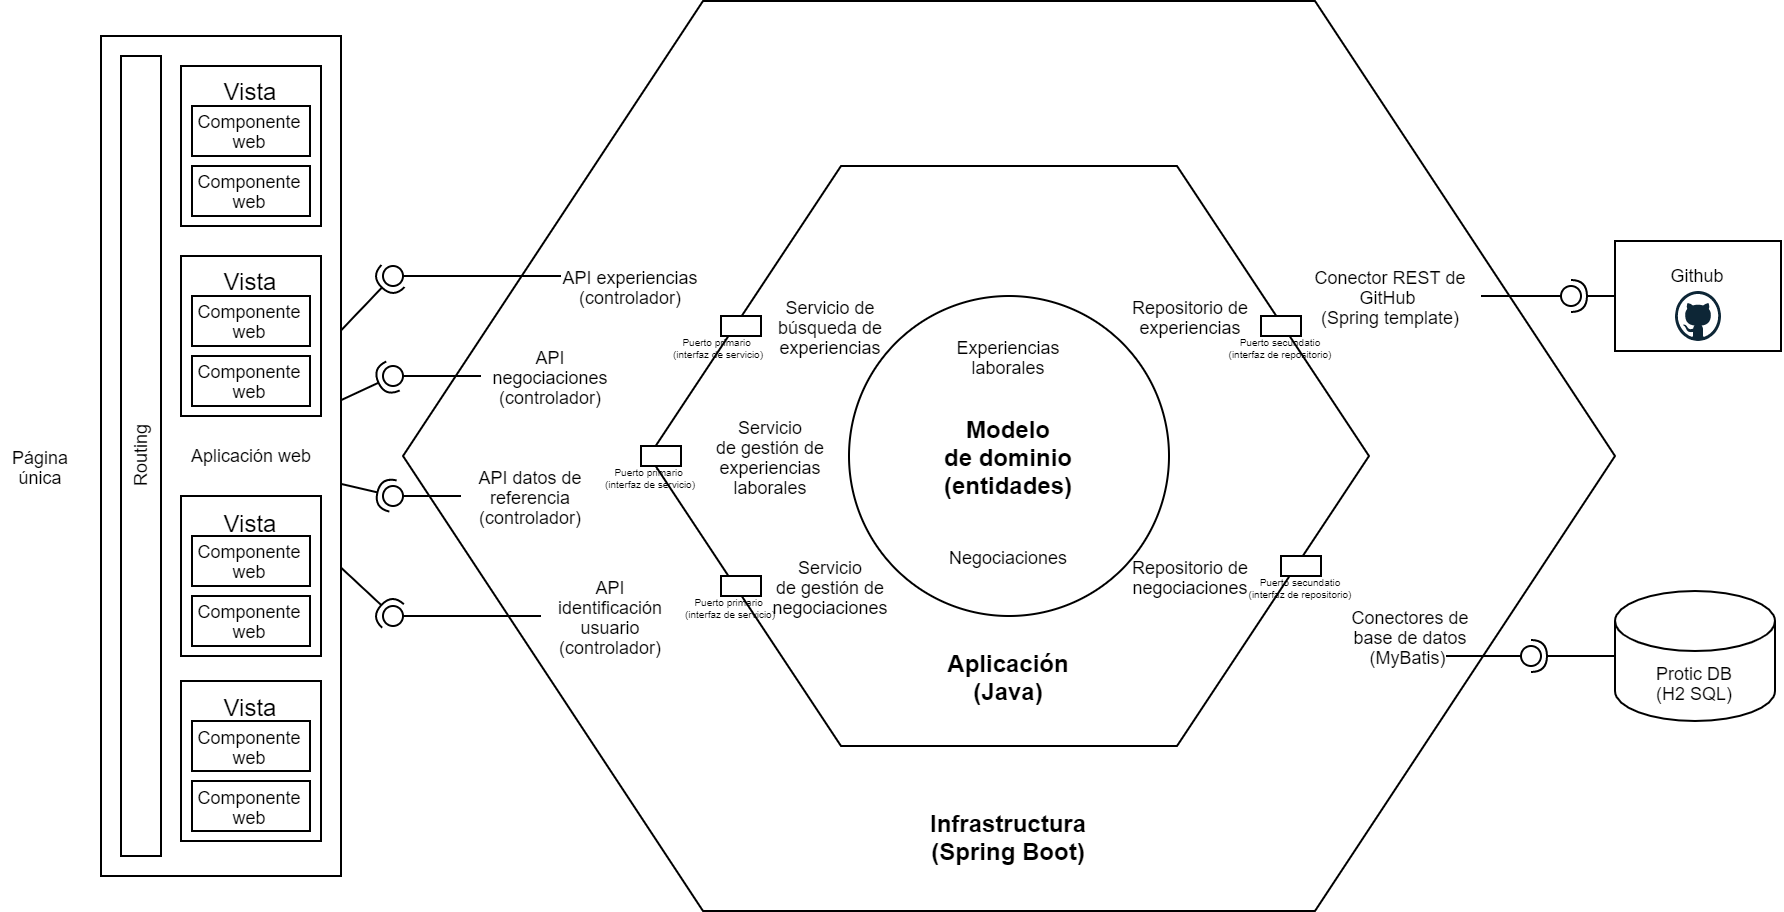
\includegraphics[width=15cm, keepaspectratio]{img/Arquitectura_hexagonal.png}
  \caption{Esquema de la arquitectura general.}\label{fig:general_architecture}
\end{figure}

\section{Modelo de dominio}
\label{sec:domain_model_impl}
A continuación se describe la implementación del modelo de dominio de la aplicación. Para ello esta sección se estructurará en cinco subsecciones:

	\begin{itemize}
	\item Clases e interfaces comunes: aquellas clases del modelo de dominio comunes a toda la aplicación.
	\item Objetos de valor del dominio de las experiencias laborales: clases de los objetos de valor relacionados con la entidad experiencia laboral.
	\item Entidad experiencia laboral: descripción de las clases e interfaces que constituyen la entidad experiencia laboral.
	\item Objetos de valor del dominio de las negociaciones: clases de los objetos de valor relacionados con la entidad negociación.
	\item Entidad negociación: descripción de las clases e interfaces que constituyen la entidad negociación.
	\end{itemize}

Para ayudar a visualizar la implementación del modelo de dominio se han añadido las Figuras~\ref{fig:domain_model_vo} y~\ref{fig:domain_model_entities} que representan los objetos de valor y las entidades de la aplicación respectivamente.

\begin{figure}
  \centering
  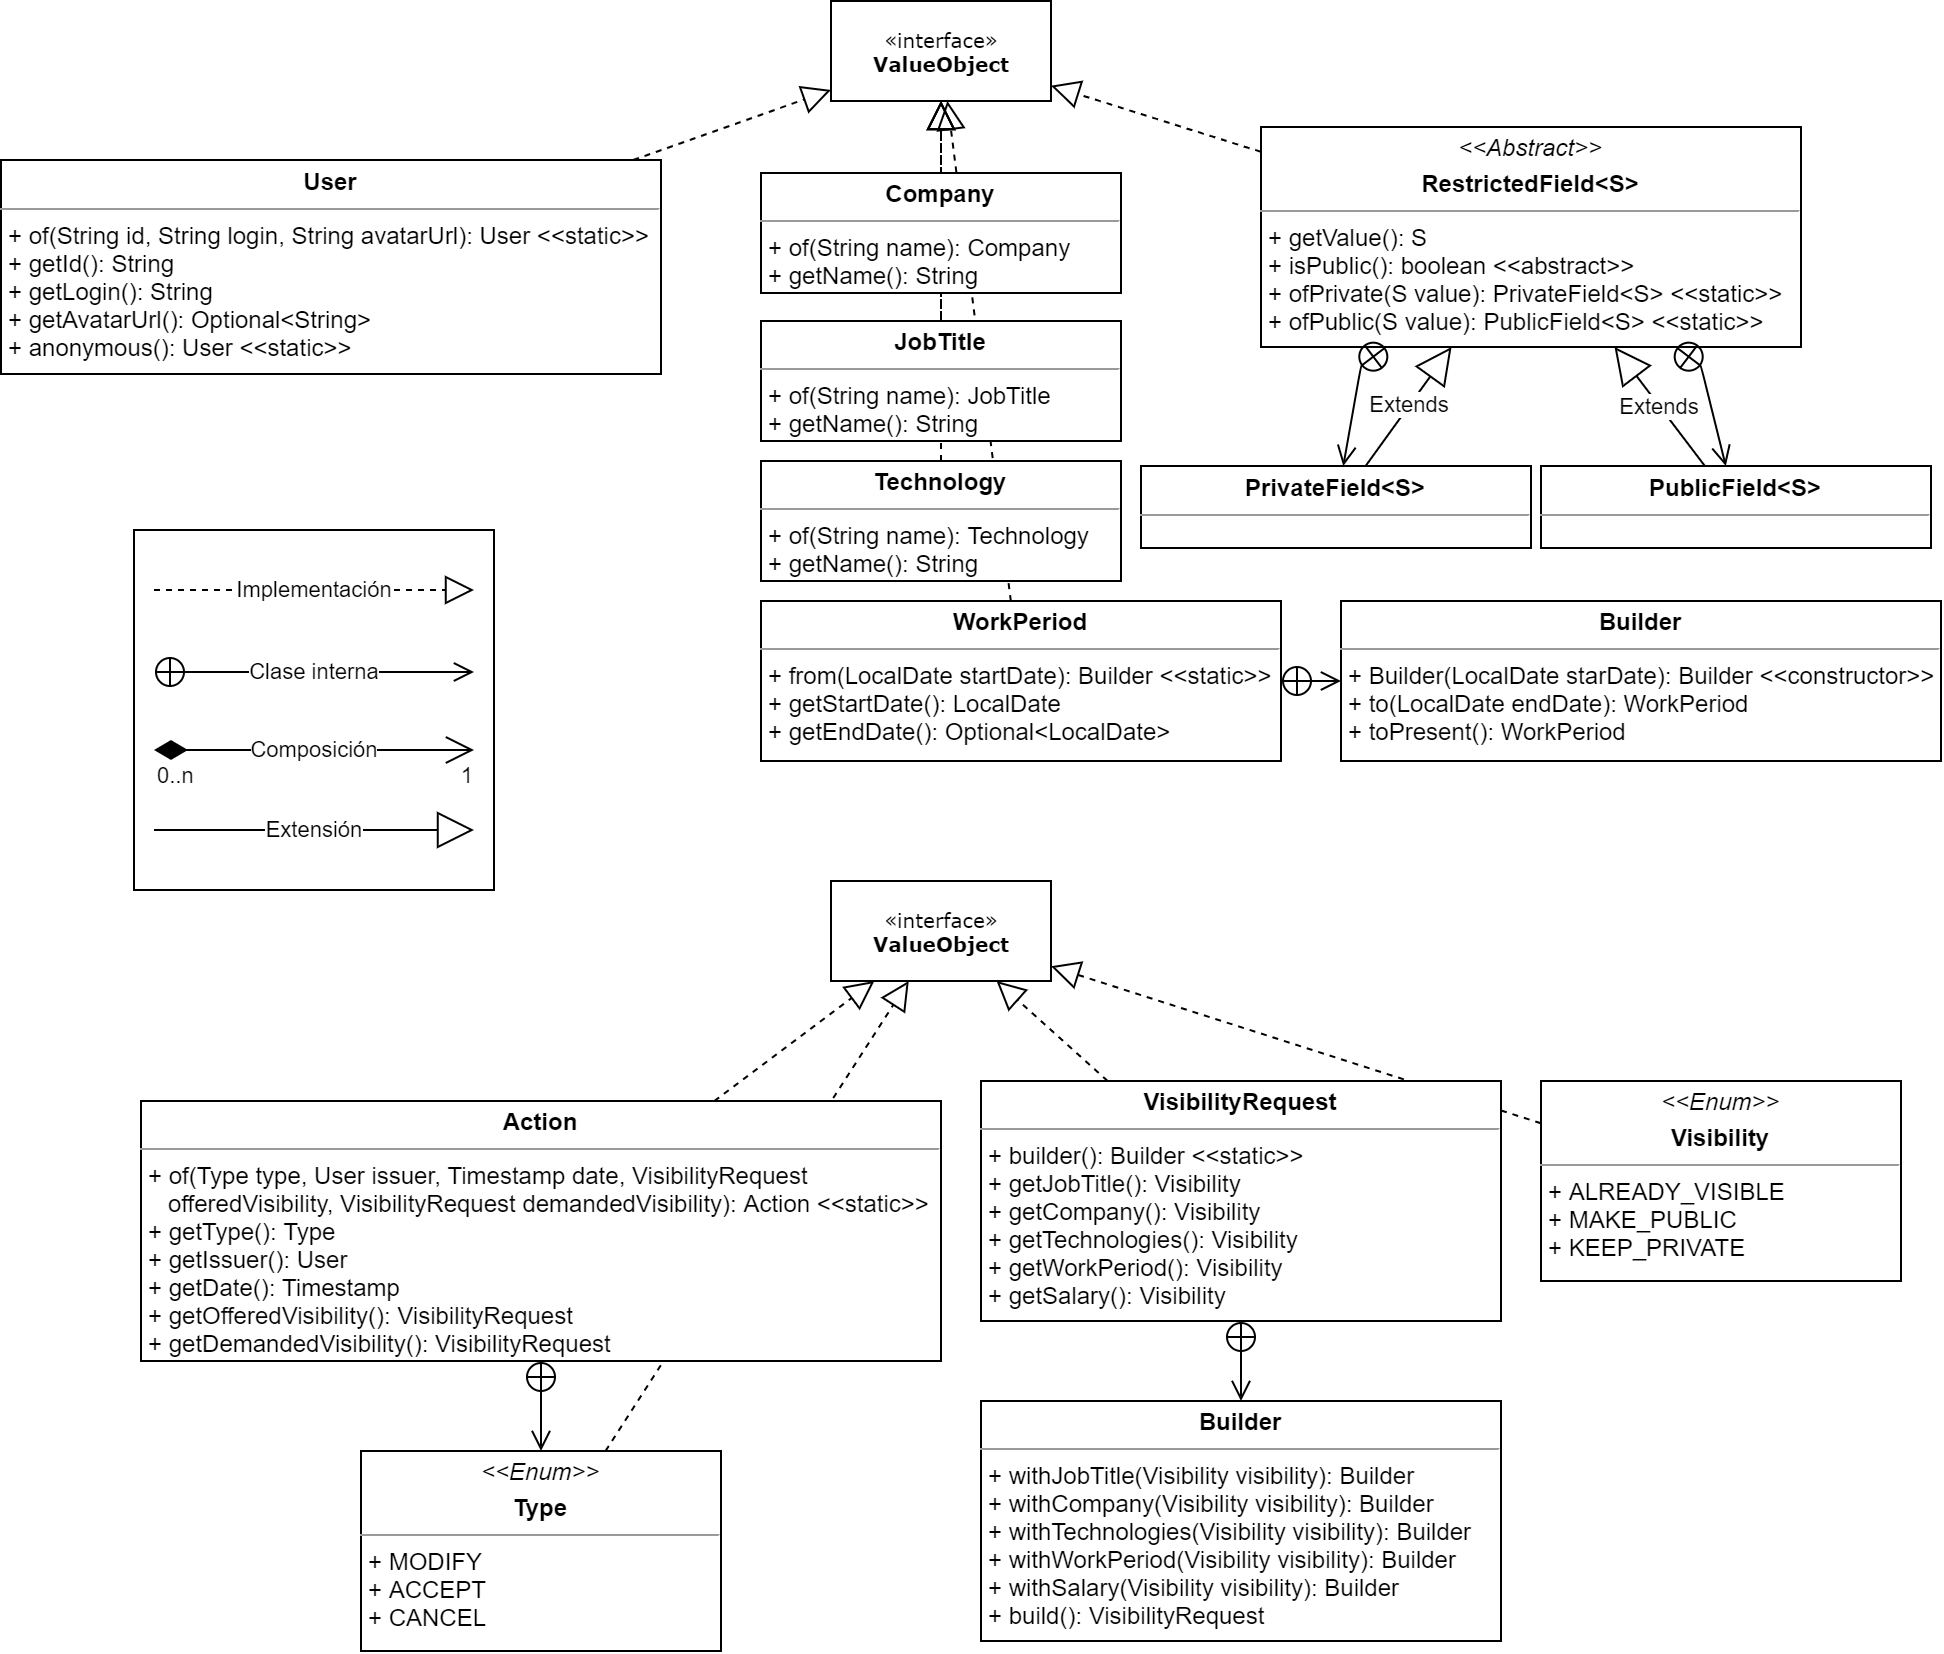
\includegraphics[width=15cm, keepaspectratio]{img/Modelo_dominio_vo.png}
  \caption{Representación de los objetos de valor del modelo de dominio.}\label{fig:domain_model_vo}
\end{figure}

\begin{figure}
  \centering
  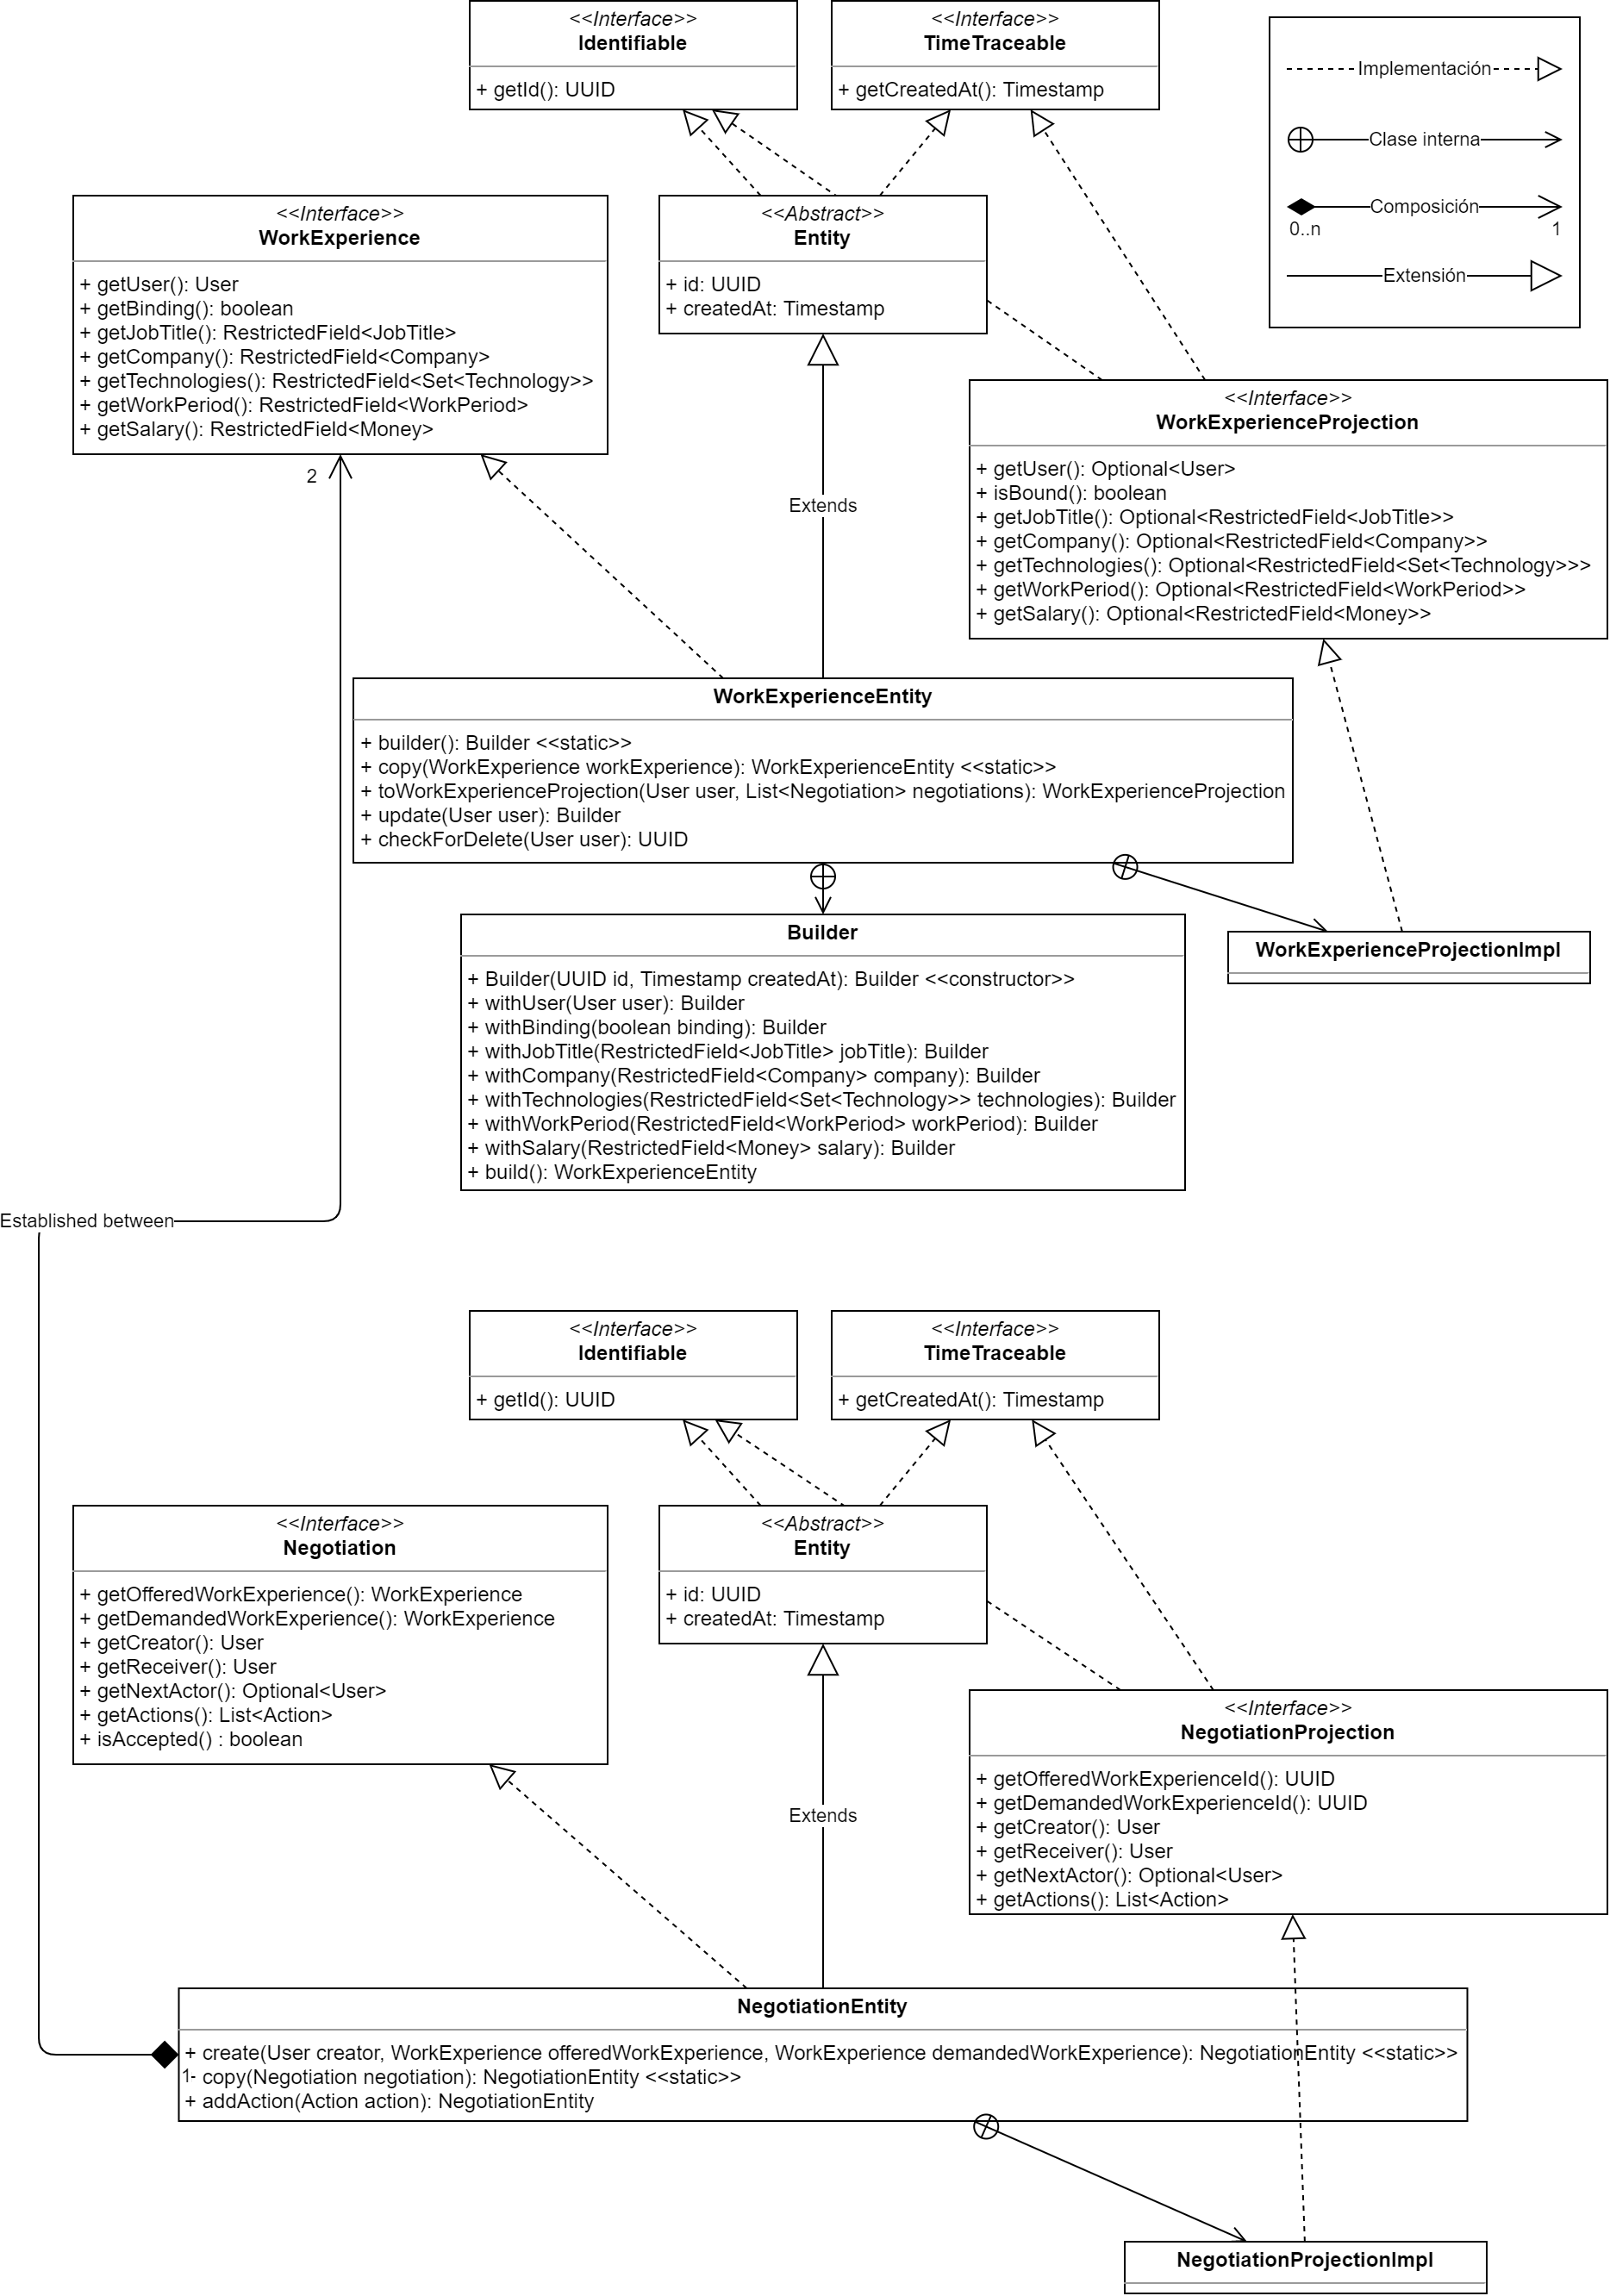
\includegraphics[width=15cm, keepaspectratio]{img/Modelo_dominio_entities.png}
  \caption{Representación de las entidades del modelo de dominio.}\label{fig:domain_model_entities}
\end{figure}

\subsection{Clases e interfaces comunes}
\label{subsec:common_classes}
Son las clases e interfaces utilizadas en todo el modelo de dominio de la aplicación. Se listan a continuación:

	\begin{itemize}
	\item \textbf{Identifiable:} Interfaz que implementan aquellas clases que se pueden identificar mediante un identificador único de tipo \emph{UUID}.
	\item \textbf{TimeTraceable:} Interfaz que implementan aquellas clases que tienen una fecha de creación.
	\item\textbf{Entity:} Clase abstracta que extienden todas las entidades del modelo de dominio. Puesto que las entidades son siempre identificables y su fecha de creación es relevante, esta clase implementa ambas interfaces \emph{Identifiable} y \emph{TimeTraceable}
	\item \textbf{ValueObject:} Interfaz que implementan aquellas clases que son objetos de valor, es decir, aquellas clases que representan tipos de datos inmutables. Esta interfaz no tiene funcionalidad, su propósito es únicamente semántico.
	\item \textbf{User:} Objeto de valor que representa a un usuario de la aplicación. Contiene como datos el idetificador del usuario en GitHub, su nombre de usuario y la URL de su avatar.
	\end{itemize}

\subsection{Objetos de valor del dominio de las experiencias laborales}
\label{subsec:work_experience_value_objects}
Los objetos de valor del dominio de la experiencia laboral son clases que reprensetan aquellos tipos de datos estáticos de los que se compone la información de la experiencia laboral.
Su propósito es doble, por una parte aportan semántica al tipado de los atributos de la entidad experiencia laboral, por otra facilitan implementar las validaciones necesarias para construir estos atributos.
Se listan a continuación:

	\begin{itemize}
	\item \textbf{Company:} Representa la empresa donde tuvo lugar la experincia laboral.
	\item \textbf{JobTitle:} Representa el puesto de trabajo de la experiencia laboral.
	\item\textbf{Technology:} Representa una tecnología que se manejó dentro de una experiencia laboral.
	\item \textbf{WorkPeriod:} Representa un periodo laboral con fecha de inicio y que puede tener o no fecha de fin. Se construye a través de una clase \emph{Builder} que permite la creación de periodos laborales concluidos o que duran hasta la actualidad.
	\item \textbf{RestrictedField:} Es una clase genérica cuyo propósito es envolver a un objeto de valor de los tipos anteriores, añadiéndole en cada caso la visibilidad pública o privada. Para ello tiene dos extensiones llamadas \emph{PrivateField} y \emph{PublicField}.
	Se puede construir a partir de dos métodos estáticos que aceptan un objeto de valor como parámetro y devuelven un objeto de una de las dos extensiones que contiene al objeto de valor.
	\end{itemize}



\subsection{Entidad experiencia laboral}
\label{subsec:work_experience_entity}
Aquí se describen las clases e interfaces que están relacionadas con el concepto de experiencia laboral como entidad de la aplicación:

	\begin{itemize}
	\item \textbf{WorkExperienceEntity:} Clase principal, representa directamente la entidad experiencia laboral.
	Se compone principalmente de una serie de atributos finales, estos atributos tienen como tipo uno de los objetos de valor de la experiencia laboral, pero envueltos como campos restringidos.
	Estos atributos, que pueden ser públicos o privados, son el nombre del puesto de trabajo, la empresa, la lista de tecnologías utilizadas, el periodo laboral y el salario. Adicionalmente esta entidad guarda la información del usuario al que pertenece, y su decisión de vincularla o no a su perfil.
	Esta entidad tiene en sus métodos la lógica de negocio necesaria para:
		\begin{itemize}
		\item Actualizar su información comprobando previamente que el usuario que la actualiza es dueño de la entidad experiencia laboral que trata de actualizar.
		\item Comprobar que un usuario que trata de borrar la entidad es dueño de esta para permitirlo o impedirlo en caso contrario.
		\item Generar una proyección de la propia entidad para un usuario concreto que trata de consultarla, con los campos que el usuario solicitante no tiene permiso para ver omitidos.
		\end{itemize}
	\item \textbf{WorkExperienceProjection:} Esta interfaz se devuelve en las consultas de experiencias laborales de la aplicación, en lugar de las propias entidades. Su utilidad es la de omitir todos aquellos atributos que el usuario solicitante no tiene permiso para ver. Para ello, la entidad genera proyecciones de este tipo siguiendo las siguientes reglas:
		\begin{itemize}
		\item Un atributo siempre es visible para el poseedor de la experiencia laboral.
		\item Un atributo es visible para cualquier usuario si es público.
		\item Un atributo privado solo es visible para un usuario que no sea poseedor de la entidad, si existe para esta entidad alguna negociación entre el solicitante y el poseedor en estado aceptado que habilite el atributo.
		\item El usuario poseedor de la entidad es siempre visible a sí mismo.
		\item El usuario poseedor de la entidad es solo visible para otros usuarios si vinculó la experiencia laboral a su perfil. En caso contrario se mostrará como anónimo.
		\end{itemize}
	\item \textbf{WorkExperience:} Esta interfaz es implementada por la entidad. Provee los métodos de acceso a sus atributos, pero no contiene los métodos de negocio de la entidad. De esta forma se impide que fuera de la capa de aplicación se trate de invocar métodos de negocio.
	\end{itemize}


\subsection{Objetos de valor del dominio de las negociaciones}
\label{subsec:negotiation_value_objects}
Los objetos de valor del dominio de las negociaciones son clases que reprensetan aquellos tipos de datos estáticos que conforman una negociaciónl.
Su propósito es contener la información relativa al histórico de la negociación y la visibilidad que los usuarios ofrecen y solicitan en relación a las experiencias laborales.
Se listan a continuación:

	\begin{itemize}
	\item \textbf{Visibility:} Tipo enumerado que reprensenta un cambio de visibilidad sobre un campo. Tiene tres posibles valores:
		\begin{itemize}
		\item \textbf{MAKE\_PUBLIC:} En relación a un campo de una experiencia laboral indica que se solicita que se convierta en público.
		\item \textbf{KEEP\_PRIVATE:} En relación a un campo de una experiencia laboral indica que no se solicita que el campo se convierta en público, sino que se mantenga privado.
		\item \textbf{ALREADY\_VISIBLE:} En relación a un campo de una experiencia laboral indica que el campo ya era público previamente a la negociación.
		\end{itemize}
	\item \textbf{VisibilityRequest:} Representa una solicitud de visibilidad sobre una experiencia laboral. Contiene un atributo por campo de la experiencia laboral, de tipo \emph{Visibility} indicando que política de visibilidad se quiere establecer sobre el campo.
	\item \textbf{Action:} Representa una acción en el histórico de una negociación. Las acciones pueden ser de tipo \emph{modificación, aceptación y cancelación} en función de si modifican la negociación o la aceptan o cancelan.
	Cada acción tiene una referencia al usuario que la ejecuta.
	Cada acción tiene ligadas la oferta de visibilidad sobre la experiencia laboral ofrecida y la solicitud de visibilidad sobre la oferta laboral solicitada, ambas del tipo \emph{VisibilityRequest}.
	\end{itemize}


\subsection{Entidad negociación}
\label{subsec:negotiation_entity}
Aquí se describen las clases e interfaces que están relacionadas con el concepto de negociaciónl como entidad de la aplicación:

	\begin{itemize}
	\item \textbf{NegotiationEntity:} Clase principal, representa directamente la entidad negociación.
	Se compone de:
		\begin{itemize}
		\item La referencia al usuario creador de la negociación.
		\item La referencia al usuario receptor de la negociación.
		\item La experiencia laboral que el usuario creador de la negociación ofreció.
		\item La experiencia laboral que el usuario creador de la negociación solictó al usuario receptor.
		\item El histórico de acciones que sucedieron durante la negociación.
		\item La referencia al usuario que debe dar el siguiente paso en la negociación si esta está activa.
		\end{itemize}
	Esta entidad tiene en sus métodos la lógica de negocio necesaria para comprobar que un usuario que añade una acción a la negociación tiene permiso para hacerlo, comprobando si es el siguiente actor de la negociación.
	\item \textbf{NegotiationProjection:} Esta interfaz se devuelve en las consultas de negociaciones de la aplicación, en lugar de las propias entidades.
	 Su utilidad es la de omitir todas las referencias de la negociación a un usuario cuando este no tiene vinculada con su perfil la experiencia laboral sobre la que se estable la negociación, de forma que el otro usuario no pueda conocer en ningún momento su identidad mientras negocia con él.
	\item \textbf{Negotiation:} Esta interfaz es implementada por la entidad. Provee los métodos de acceso a sus atributos, pero no contiene los métodos de negocio de la entidad. De esta forma se impide que fuera de la capa de aplicación se trate de invocar métodos de negocio.
	\end{itemize}



\section{Modelo de datos}
\label{sec:data_model}
Para explicar el modelo de datos de la aplicación se dará una breve descripción de cada una de las tablas que lo componen. La explicación se apoyará en el diagrama de la Figura~\ref{fig:data_model}

\begin{figure}
  \centering
  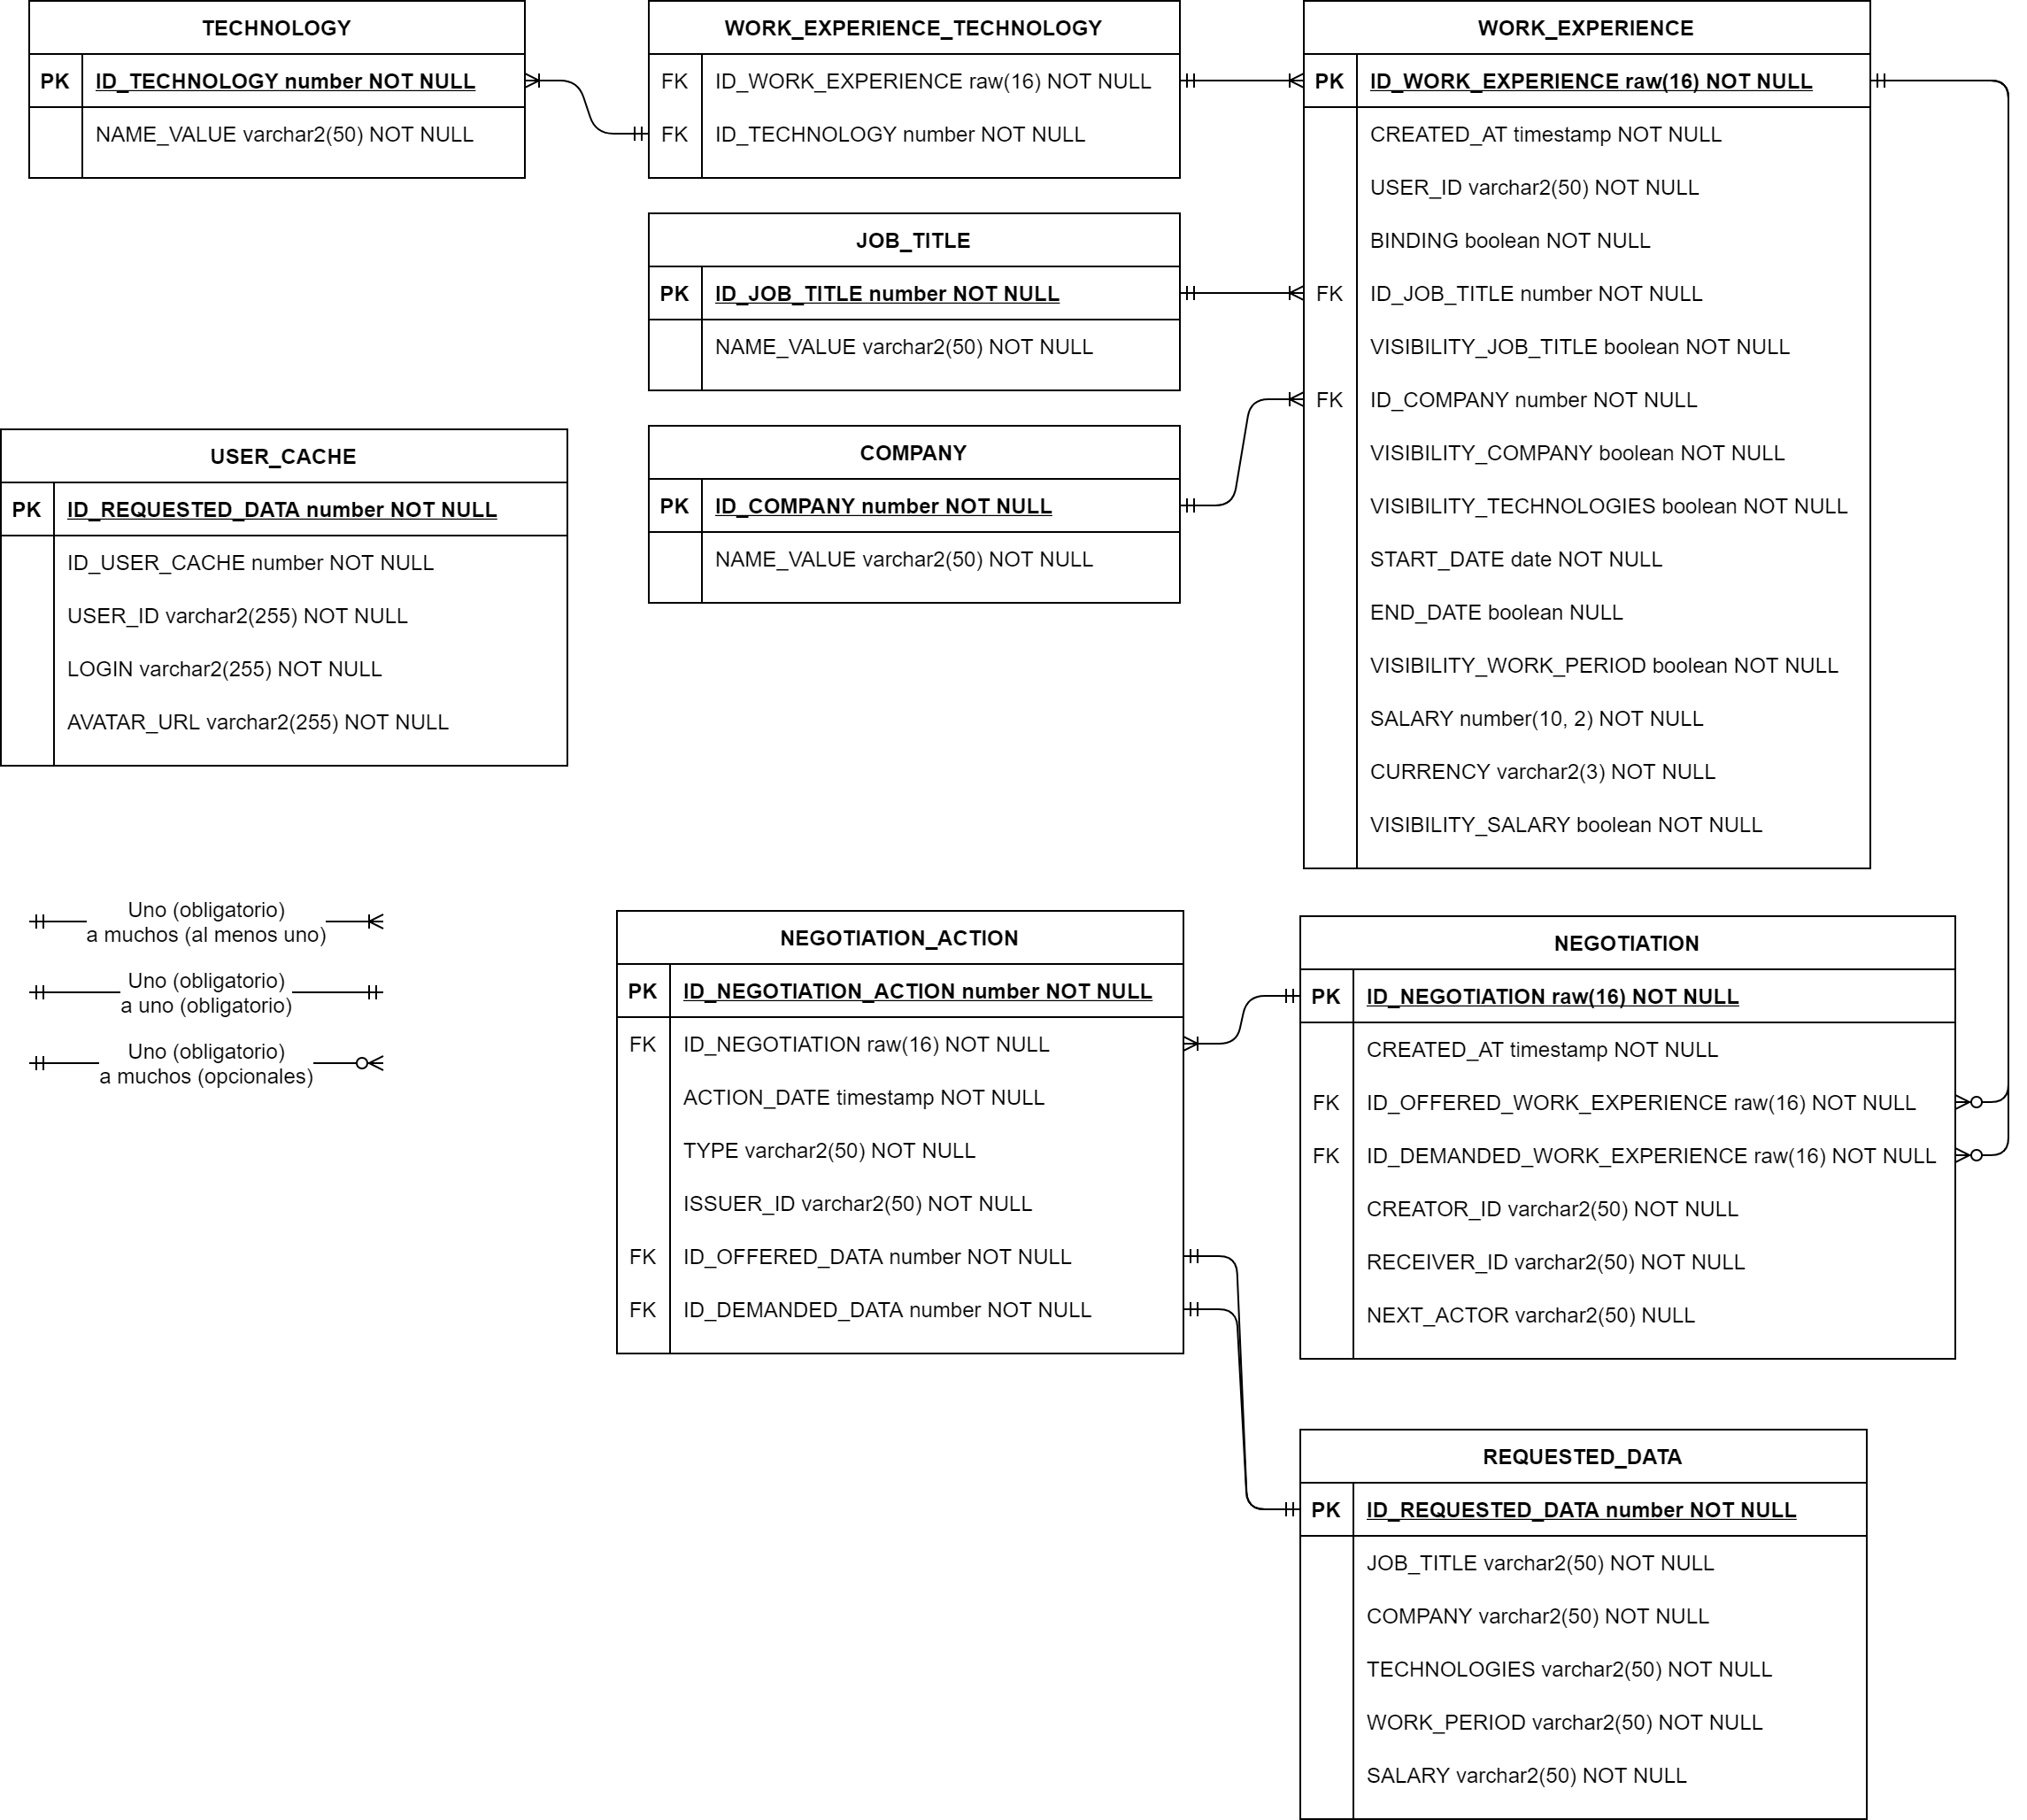
\includegraphics[width=15cm, keepaspectratio]{img/Modelo_datos.png}
  \caption{Diagrama de entidad relación del modelo de datos.}\label{fig:data_model}
\end{figure}


	\begin{itemize}
	\item \textbf{Tabla WORK\_EXPERIENCE:} En ella se alamacenan los datos relativos a cada experiencia laboral perteneciente a los usuarios.
	Contiene el identificador único de la experiencia laboral, su fechar de creación, el identificador del usuario al que pertenece la experiencia, el indicador de si la experiencia extá vinculada o no al perfil del usuario.
	Además, para cada campo de la experiencia laboral, esta tabla contiene:
		\begin{itemize}
		\item Puesto de trabajo: la visibilidad (privada o pública) del campo y una referencia a la tabla \emph{JOB\_TITLE} que contiene el puesto de trabajo.
		\item Empresa: la visibilidad (privada o pública) del campo y una referencia a la tabla \emph{COMPANY} que contiene el nombre de la empresa.
		\item Tecnologías: la visibilidad (privada o pública) del campo. La tabla \emph{WORK\_ EXPERIENCE\_TECHNOLOGY} puede contener varias referencias a esta tabla, una por tecnología asociada a la experiencia laboral.
		\item Período laboral: la visibilidad (privada o pública) del campo y las fechas de inicio y fin de la experiencia laboral, siendo la última nula si la experiencia dura hasta la actualidad.
		\item Salario: la visibilidad (privada o pública) del campo y la cuantía del salario bruto anual, además del código ISO de la moneda.
		\end{itemize}
	\item \textbf{Tabla JOB\_TITLE:} Contiene los nombres de los puestos de trabajo relacionados con las experiencias laborales.
	\item \textbf{Tabla COMPANY:} Contiene los nombres de las empresas relacionadas con las experiencias laborales.
	\item \textbf{Tabla WORK\_EXPERIENCE\_TECHNOLOGY:} Relaciona las experincias laborales con las tecnologías utilizadas en cada una de ellas, mediante una relación de muchas a muchas.
	\item \textbf{Tabla TECHNOLOGY:} Contiene los nombres de las tecnologías relacionadas con las experiencias laborales.
	\item \textbf{Tabla NEGOTIATION:} En ella se almacenan los datos relativos a las negociaciones.
	Contiene el identificador único de la negociación, su fecha de creación, una referencia a la experiencia laboral ofrecida en la negociación y otra a la experiencia laboral solicitada, el identificador del usuario creador de la negociación y del usuario receptor, y el identificador del usuario que será el siguiente actor en la negociación, si aplica.
	\item \textbf{Tabla NEGOTIATION\_ACTION:} En ella se almacena el histórico de acciones que han ido transcurriendo para cada negociación.
	Cada registro contiene la referencia a la negociación sobre la que se aplicó la acción, la fecha en la que se aplicó, el tipo de acción (modificación, aceptación o cancelación), el identificador del usuario que realizó la acción,
	y las referencias a la tabla \emph{REQUESTED\_DATA} donde se almacenan la visibilidad a aplicar a cada uno de los campos de la experiencia ofrecida y de la experiencia solicitada.
	\item \textbf{Tabla REQUESTED\_DATA:} En ella se almacenan los posibles valores de la visibilidad de los campos para una experiencia laboral en negociación, siendo estos "manetener privado", "hacer público" o "ya público".
	\item \textbf{Tabla USER\_CACHE:} En esta tabla se almacena la información de los usuarios que se obtiene de GitHub, para evitar realizar peticiones HTTP para información de usuarios que ya se ha obtenido en el pasado.
	\end{itemize}


\section{Diseño del API}
\label{sec:api_desing}
En esta sección se describirá el API REST de la aplicación en cuatro grupos de puntos de API según su clasifiación funcional:

		\begin{itemize}
		\item Puntos de API de sesión: aquellos relacionados con la sesión del usuario.
		\item Puntos de API de datos de referencia: aquellos que se utilizan para consultar puestos de trabajo, empresas y tecnologías que ya se dieron de alta en la aplicación.
		\item Puntos de API de experiencias laborales: aquellos relacionados con operaciones sobre la entidad experiencia laboral.
		\item Puntos de API de negociaciones: aquellos relacionados con operaciones sobre la entidad negociación.
		\end{itemize}

\subsection{Puntos de API de sesión}
\label{subsec:session_endpoints}
Es el conjunto de dos puntos de API que proveen operaciones relacionadas con la sesión del usuario:

\subsubsection{Punto de API de obtención de usuario}
\label{subsec:get_user}
Este punto de API se utiliza para obtener la información del usuario que encuentra en sesión.
Las solicitudes se envían metidante el método \emph{GET} al recurso de la aplicación \emph{/user}.
A continuación se muestra un ejemplo de llamada al punto de API:

			{\footnotesize
			\begin{verbatim}
			-- Solicitud
			GET /user

			-- Respuesta
			200 OK
			{
			    "id": "1",
			    "login": "mojombo",
			    "avatarUrl": "https://avatars.githubusercontent.com/u/1?v=4"
			}
			\end{verbatim}
			}

\subsubsection{Punto de API de cierre de sesión}
\label{subsec:get_user}
Este punto de API se utiliza para invalidar la sesión del usuario en un cierre de sesión.
Las solicitudes se envían metidante el método \emph{GET} al recurso de la aplicación \emph{/user/logout}.
A continuación se muestra un ejemplo de llamada al punto de API:

			{\footnotesize
			\begin{verbatim}
			-- Solicitud
			GET /user/logout

			-- Respuesta
			200 OK
			\end{verbatim}
			}

\subsection{Puntos de API de datos de referencia}
\label{subsec:reference_endpoints}
Es el conjunto de tres puntos de API que se utilizan para proveer listados de información preexistente para las experencias laborales.
Se utilizan principalmente para alimentar componentes de tipo combo en la interfaz de usuario:

\subsubsection{Punto de API de datos de puesto de trabajo}
\label{subsec:get_data_job_titles}
Este punto de API se utiliza para obtener la lista de nombres de puestos de trabajo que ya existen en la aplicación.
Las solicitudes se envían metidante el método \emph{GET} al recurso de la aplicación \emph{/data/job-titles}.
La solicitud acepta un parámetro de consulta llamado \emph{name} cuyo valor permite filtrar aquellos elementos de la lista que lo contienen en su nombre:
A continuación se muestra un ejemplo de llamada al punto de API:

			{\footnotesize
			\begin{verbatim}
			-- Solicitud
			GET /data/job-titles?name=pro

			-- Respuesta
			200 OK
			{
			    "data": [
			        "ANALISTA/PROGRAMADOR",
			        "DISEÑADOR DE PROCESOS",
			        "PRODUCT OWNER",
			        "PROGRAMADOR"
			    ]
			}
			\end{verbatim}
			}

\subsubsection{Punto de API de datos de empresas}
\label{subsec:get_data_companies}
Este punto de API se utiliza para obtener la lista de nombres de empresas que ya existen en la aplicación.
Las solicitudes se envían metidante el método \emph{GET} al recurso de la aplicación \emph{/data/companies}.
La solicitud acepta un parámetro de consulta llamado \emph{name} cuyo valor permite filtrar aquellos elementos de la lista que lo contienen en su nombre:
A continuación se muestra un ejemplo de llamada al punto de API:

			{\footnotesize
			\begin{verbatim}
			-- Solicitud
			GET /data/companies?name=in

			-- Respuesta
			200 OK
			{
			    "data": [
			        "ARQUIMEA INGENIERÍA",
			        "INDRA",
			        "ING"
			    ]
			}
			\end{verbatim}
			}

\subsubsection{Punto de API de datos de tecnologías}
\label{subsec:get_data_job_technologies}
Este punto de API se utiliza para obtener la lista de nombres de tecnologías que ya existen en la aplicación.
Las solicitudes se envían metidante el método \emph{GET} al recurso de la aplicación \emph{/data/technologies}.
La solicitud acepta un parámetro de consulta llamado \emph{name} cuyo valor permite filtrar aquellos elementos de la lista que lo contienen en su nombre:
A continuación se muestra un ejemplo de llamada al punto de API:

			{\footnotesize
			\begin{verbatim}
			-- Solicitud
			GET /data/technologies?name=j

			-- Respuesta
			200 OK
			{
			    "data": [
			        "DJANGO",
			        "JAVA",
			        "JAVA 11",
			        "JAVASCRIPT",
			        "JQUERY",
			        "VUE JS"
			    ]
			}
			\end{verbatim}
			}

\subsection{Puntos de API de experiencias laborales}
\label{subsec:work_experience_endpoints}
Es el conjunto de dos puntos de API que proveen operaciones sobre la entidad experiencia laboral.

\subsubsection{Punto de API de creación de experiencia laboral}
\label{subsec:post_work_experience}
Este punto de API se utiliza para crear una nueva experiencia laboral.
Las solicitudes se envían metidante el método \emph{POST} al recurso de la aplicación \emph{/work-experience}.
El cuerpo de la solicitud contiene la información acerca de la experiencia laboral a crear en formato JSON.
La respuesta contiene el identificador único de la nueva experiencia laboral.
A continuación se muestra un ejemplo de llamada al punto de API:

			{\footnotesize
			\begin{verbatim}
			-- Solicitud
			POST /work-experience
			{
			    "binding": true,
			    "jobTitle": {
			        "public": true,
			        "content": "Analista/Desarrollador"
			    },
			    "company": {
			        "public": true,
			        "content": "Indra"
			    },
			    "technologies": {
			        "public": true,
			        "content": [
			            "Java",
			            "Spring"
			        ]
			    },
			    "workPeriod": {
			        "public": true,
			        "content": {
			            "startDate": "2020-04-10",
			            "endDate": "2021-04-11"
			        }
			    },
			    "salary": {
			        "public": true,
			        "content": {
			            "value": 36000,
			            "currency": "EUR"
			        }
			    }
			}

			-- Respuesta
			200 OK
			{
			    "id": "99784c87-70d0-43cc-a340-aa28a19cb8a3"
			}
			\end{verbatim}
			}

\subsubsection{Punto de API de obtención de experiencia laboral por identificador}
\label{subsec:get_work_experience_id}
Este punto de API se utiliza para recuperar una experiencia laboral por su identificador único.
Las solicitudes se envían metidante el método \emph{GET} al recurso de la aplicación \emph{/work-experience/\{id\}}, donde \emph{id} es el identificador de la experiencia laboral a recuperar.
La respuesta contiene los datos de la experiencia laboral, con los filtros de visibilidad aplicados según el usuario solicitante.
A continuación se muestra un ejemplo de llamada al punto de API:

			{\footnotesize
			\begin{verbatim}
			-- Solicitud
			GET /work-experience/99784c87-70d0-43cc-a340-aa28a19cb8a3

			-- Respuesta
			200 OK
			{
			    "id": "99784c87-70d0-43cc-a340-aa28a19cb8a3",
			    "user":{
			        "id": "5689851",
			        "login": "vicengg",
			        "avatarUrl": "https://avatars.githubusercontent.com/u/5689851?v=4"
			    },
			    "binding": true,
			    "jobTitle":{
			        "content": "ANALISTA/DESARROLLADOR",
			        "public": true
			    },
			    "company":{
			        "content": "INDRA",
			        "public": true
			    },
			    "technologies":{
			        "content":[
			            "JAVA",
			            "SPRING"
			        ],
			        "public": true
			    },
			    "workPeriod":{
			        "content":{
			            "startDate": "2020-04-10",
			            "endDate": "2021-04-11"
			        },
			        "public": true
			    },
			    "salary":{
			        "content":{
			            "value": 3.6E+4,
			            "currency": "EUR"
			        },
			        "public": true
			    }
			}
			\end{verbatim}
			}

\subsubsection{Punto de API de búsqueda de experiencias laborales}
\label{subsec:get_work_experience}
Este punto de API se utiliza para buscar experiencias laborales filtrando por su contenido.
Las solicitudes se envían metidante el método \emph{GET} al recurso de la aplicación \emph{/work-experience}.
La solicitud admite varios parámetros de consulta que filtran el resultado:
		\begin{itemize}
		\item \emph{scope}: Indica si se solicitan todas las experiencias laborales (\emph{scope=all}), las del usuario (\emph{scope=own}) o las del resto de usuarios (\emph{scope=foreign}).
		Su valor por defecto es \emph{all}.
		\item \emph{jobTitle}: Al asignar un cadena de caracteres a este filtro, solo se devolveran aquellas experiencias que contengan esa en el nombre del puesto de trabajo.
		\item \emph{company}: Al asignar un cadena de caracteres a este filtro, solo se devolveran aquellas experiencias que contengan esa en el nombre de la empresa.
		\item \emph{technologies}: Al asignar múltiples cadenas de caracteres a este filtro, solo se devolveran aquellas experiencias que contengan esas cadenas en su lista de tecnologías.
		\item \emph{startDate}: Enviar este filtro hará que solo las experiencias laborales que iniciaron después de la fecha indicada estén presentes en la respuesta.
		\item \emph{endDate}: Enviar este filtro hará que solo las experiencias laborales que iniciaron antes de la fecha indicada estén presentes en la respuesta.
		\item \emph{minSalary}: Enviar este filtro hará que solo las experiencias laborales con un salario superior al indicado estén presentes en la respuesta.
		\item \emph{maxSalary}: Enviar este filtro hará que solo las experiencias laborales con un salario inferior al indicado estén presentes en la respuesta.
		\end{itemize}
La respuesta contiene un listado de experiencias laborales, con los filtros de visibilidad aplicados según el usuario solicitante.
A continuación se muestra un ejemplo de llamada al punto de API:

			{\footnotesize
			\begin{verbatim}
			-- Solicitud
			GET /work-experience?scope=own&jobTitle=programador&company=arquimea
			&technologies=java&technologies=angular&startDate=2015-01-01
			&endDate=2018-01-01&minSalary=5000&maxSalary=20000

			-- Respuesta
			200 OK
			{
			    "result": [{
			        "id": "60219d70-ae4d-11eb-8529-0242ac130003",
			        "user":{
			            "id": "5689851",
			            "login": "vicengg",
			            "avatarUrl": "https://avatars.githubusercontent.com/u/5689851?v=4"
			        },
			        "binding": true,
			        "jobTitle":{
			            "content": "PROGRAMADOR",
			            "public": true
			        },
			        "company":{
			            "content": "ARQUIMEA INGENIERÍA",
			            "public": true
			        },
			        "technologies":{
			            "content":[
			                "JAVASCRIPT",
			                "JAVA",
			                "SPRING",
			                "JQUERY",
			                "ANGULAR"
			            ],
			            "public": true
			        },
			        "workPeriod":{
			            "content":{
			                "startDate": "2015-03-01",
			                "endDate": "2017-07-01"
			            },
			            "public": true
			        },
			        "salary":{
			            "content":{
			                "value": 1.1E+4,
			                "currency": "EUR"
			            },
			            "public": false
			        }
			    }]
			}
			\end{verbatim}
			}

\subsubsection{Punto de API de actualización de experiencia laboral}
\label{subsec:put_work_experience}
Este punto de API se utiliza para actualizar una experiencia laboral.
Las solicitudes se envían metidante el método \emph{POST} al recurso de la aplicación \emph{/work-experience/\{id\}}, donde \emph{id} es el identificador de la experiencia laboral a actualizar.
El cuerpo de la solicitud contiene la información acerca de la experiencia laboral a actualizar en formato JSON.
A continuación se muestra un ejemplo de llamada al punto de API:

			{\footnotesize
			\begin{verbatim}
			-- Solicitud
			PUT /work-experience/99784c87-70d0-43cc-a340-aa28a19cb8a3
			{
			    "binding": true,
			    "jobTitle": {
			        "public": true,
			        "content": "Analista/Desarrollador"
			    },
			    "company": {
			        "public": true,
			        "content": "Indra"
			    },
			    "technologies": {
			        "public": true,
			        "content": [
			            "Java",
			            "Spring"
			        ]
			    },
			    "workPeriod": {
			        "public": true,
			        "content": {
			            "startDate": "2020-04-10",
			            "endDate": "2021-04-11"
			        }
			    },
			    "salary": {
			        "public": true,
			        "content": {
			            "value": 36000,
			            "currency": "EUR"
			        }
			    }
			}

			-- Respuesta
			200 OK
			\end{verbatim}
			}

\subsubsection{Punto de API de borrado de experiencia laboral}
\label{subsec:delete_work_experience}
Este punto de API se utiliza para borrar una experiencia laboral.
Las solicitudes se envían metidante el método \emph{DELETE} al recurso de la aplicación \emph{/work-experience/\{id\}}, donde \emph{id} es el identificador de la experiencia laboral a borrar.
A continuación se muestra un ejemplo de llamada al punto de API:

			{\footnotesize
			\begin{verbatim}
			-- Solicitud
			DELETE /work-experience/99784c87-70d0-43cc-a340-aa28a19cb8a3

			-- Respuesta
			200 OK
			\end{verbatim}
			}

\subsection{Puntos de API de negociaciones}
\label{subsec:negotiation_endpoints}
Es el conjunto de dos puntos de API que proveen operaciones sobre la entidad negociación.

\subsubsection{Punto de API de creación de negociación}
\label{subsec:post_work_experience}
Este punto de API se utiliza para crear una nueva negociación.
Las solicitudes se envían metidante el método \emph{POST} al recurso de la aplicación \emph{/negotiation}.
El cuerpo de la solicitud contiene las referencias a las experiencias laborales entre las que se establece la negociación.
La respuesta contiene el identificador único de la nueva negociación.
A continuación se muestra un ejemplo de llamada al punto de API:

			{\footnotesize
			\begin{verbatim}
			-- Solicitud
			POST /negotiation
			{
			    "offeredWorkExperienceId": "4c714c8e-9d5f-11eb-a8b3-0242ac130003",
			    "demandedWorkExperienceId": "b6b3705e-9e04-11eb-a8b3-0242ac130003"
			}

			-- Respuesta
			200 OK
			{
			    "id": "958961ae-deaa-484f-b3a7-39bcb7ca0df0"
			}
			\end{verbatim}
			}

\subsubsection{Punto de API de agregación de acciones a una negociación}
\label{subsec:put_negotiation}
Este punto de API se utiliza para agregar una nueva acción a una negociación.
Las solicitudes se envían metidante el método \emph{PUT} al recurso de la aplicación \emph{/negotiation/\{id\}}, donde \emph{id} es el identificador de la negociación a la que se le va a agregar una nueva acción.
El cuerpo de la solicitud contiene la información de la nueva acción a añadir.
A continuación se muestra un ejemplo de llamada al punto de API:

			{\footnotesize
			\begin{verbatim}
			-- Solicitud
			PUT /negotiation/958961ae-deaa-484f-b3a7-39bcb7ca0df0/action
			{
			    "type": "accept",
			    "offeredData": {
			        "jobTitle": "make_public",
			        "company": "make_public",
			        "technologies": "make_public",
			        "workPeriod": "make_public",
			        "salary": "make_public"
			    },
			    "demandedData": {
			        "jobTitle": "make_public",
			        "company": "make_public",
			        "technologies": "make_public",
			        "workPeriod": "make_public",
			        "salary": "make_public"
			    }
			}

			-- Respuesta
			200 OK
			\end{verbatim}
			}



\subsubsection{Punto de API de obtención de negociación por identificador}
\label{subsec:get_negotiation_id}
Este punto de API se utiliza para recuperar una negociación por su identificador único.
Las solicitudes se envían metidante el método \emph{GET} al recurso de la aplicación \emph{/negotiation/\{id\}}, donde \emph{id} es el identificador de la negociación a recuperar.
La respuesta contiene los datos de la negociación, con los filtros de visibilidad aplicados a algunos campos según el usuario solicitante.
A continuación se muestra un ejemplo de llamada al punto de API:

			{\footnotesize
			\begin{verbatim}
			-- Solicitud
			GET /negotiation/958961ae-deaa-484f-b3a7-39bcb7ca0df0

			-- Respuesta
			200 OK
			{
			    "id": "958961ae-deaa-484f-b3a7-39bcb7ca0df0",
			    "offeredWorkExperienceId": "4c714c8e-9d5f-11eb-a8b3-0242ac130003",
			    "demandedWorkExperienceId": "b6b3705e-9e04-11eb-a8b3-0242ac130003",
			    "creator":{
			        "id": "5689851",
			        "login": "vicengg",
			        "avatarUrl": "https://avatars.githubusercontent.com/u/5689851?v=4"
			    },
			    "receiver":{
			        "id": "0",
			        "login": "anónimo",
			        "avatarUrl": "https://crysteland.com/wp-content/uploads/2016/12/unknown-user-460x460.png"
			    },
			    "nextActor":{
			        "id": "0",
			        "login": "anónimo",
			        "avatarUrl": "https://crysteland.com/wp-content/uploads/2016/12/unknown-user-460x460.png"
			    },
			    "actions": [{
			        "type": "MODIFY",
			        "date": "2021-05-05T13:59:15.229+00:00",
			        "offeredData":{
			            "jobTitle": "MAKE_PUBLIC",
			            "company": "MAKE_PUBLIC",
			            "technologies": "MAKE_PUBLIC",
			            "workPeriod": "MAKE_PUBLIC",
			            "salary": "MAKE_PUBLIC"
			        },
			        "demandedData":{
			            "jobTitle": "MAKE_PUBLIC",
			            "company": "MAKE_PUBLIC",
			            "technologies": "MAKE_PUBLIC",
			            "workPeriod": "MAKE_PUBLIC",
			            "salary": "MAKE_PUBLIC"
			        },
			        "issuer":{
			            "id": "5689851",
			            "login": "vicengg",
			            "avatarUrl": "https://avatars.githubusercontent.com/u/5689851?v=4"
			        }
			    }]
			}
			\end{verbatim}
			}

\subsubsection{Punto de API de obtención de negociaciones}
\label{subsec:get_negotiation}
Este punto de API se utiliza obtener las negociaciones en las cuales el usuario solicitantes está implicado.
Las solicitudes se envían metidante el método \emph{GET} al recurso de la aplicación \emph{/negotiation}.
La solicitud admite un parámetro de consulta, \emph{scope},
este parámetro indica si deben devolverse las negociaciones de las que el usuario es creador (\emph{scope=creator}) o de las que el usuario es receptor (\emph{scope=receiver}).
Por defecto su valor es(\emph{scope=creator}.
La respuesta contiene un listado de negociaciones.
A continuación se muestra un ejemplo de llamada al punto de API:

			{\footnotesize
			\begin{verbatim}
			-- Solicitud
			GET /work-experience?scope=own&jobTitle=programador&company=arquimea
			&technologies=java&technologies=angular&startDate=2015-01-01
			&endDate=2018-01-01&minSalary=5000&maxSalary=20000

			-- Respuesta
			200 OK
			{
			    "result": [			{
			        "id": "958961ae-deaa-484f-b3a7-39bcb7ca0df0",
			        "offeredWorkExperienceId": "4c714c8e-9d5f-11eb-a8b3-0242ac130003",
			        "demandedWorkExperienceId": "b6b3705e-9e04-11eb-a8b3-0242ac130003",
			        "creator":{
			            "id": "5689851",
			            "login": "vicengg",
			            "avatarUrl": "https://avatars.githubusercontent.com/u/5689851?v=4"
			        },
			        "receiver":{
			            "id": "0",
			            "login": "anónimo",
			            "avatarUrl": "https://crysteland.com/wp-content/uploads/2016/12/unknown-user-460x460.png"
			        },
			        "nextActor":{
			            "id": "0",
			            "login": "anónimo",
			            "avatarUrl": "https://crysteland.com/wp-content/uploads/2016/12/unknown-user-460x460.png"
			        },
			        "actions": [{
			            "type": "MODIFY",
			            "date": "2021-05-05T13:59:15.229+00:00",
			            "offeredData":{
			                "jobTitle": "MAKE_PUBLIC",
			                "company": "MAKE_PUBLIC",
			                "technologies": "MAKE_PUBLIC",
			                "workPeriod": "MAKE_PUBLIC",
			                "salary": "MAKE_PUBLIC"
			            },
			            "demandedData":{
			                "jobTitle": "MAKE_PUBLIC",
			                "company": "MAKE_PUBLIC",
			                "technologies": "MAKE_PUBLIC",
			                "workPeriod": "MAKE_PUBLIC",
			                "salary": "MAKE_PUBLIC"
			            },
			            "issuer":{
			                "id": "5689851",
			                "login": "vicengg",
			                "avatarUrl": "https://avatars.githubusercontent.com/u/5689851?v=4"
			            }
			        }]
			    }]
			}
			\end{verbatim}
			}

\section{Componentes web}
\label{sec:web_components}
En esta sección se describen los componentes web que se implementaron para su uso en la interfaz de usuario de la applicación.

\subsubsection{ActionDisplay}
\label{subsec:wc_action_display}
Este componente que se utiliza en la vista de detalles de una negociación se utiliza para visualizar cada una de las acciones del histórico de una negociación.
Informa de el usuario que realizó la acción, el tipo de acción que realizó, el tiempo que trancurrió desde que se realizó la acción y, en caso de que la acción sea una modificación de la negociación, la visibilidad que se ofrece y solicita entre las experiencias laborales.
Este componente se muestra en la Figura~\ref{fig:component_action_display}

\begin{figure}
  \centering
  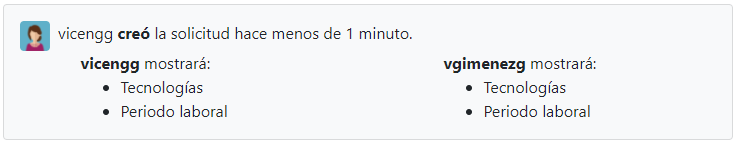
\includegraphics[width=15cm, keepaspectratio]{img/ActionDisplay.PNG}
  \caption{Ejemplo de componente web ActionDisplay.}\label{fig:component_action_display}
\end{figure}

Sus entradas son:

		\begin{itemize}
		\item \textbf{action:} Objeto con el contenido de la acción, ver definición de \emph{Action} en la Subsección~\ref{subsec:negotiation_value_objects}.
		\item \textbf{user:} Objeto que contiene la información del usuario en sesión, ver definición de \emph{User} en la Subsección~\ref{subsec:common_classes}.
		\item \textbf{isFirst:} Indica si el \emph{ActionDisplay} es o no el primer elemento de una lista, para su correcta visualización.
		\item \textbf{creator:} Objeto que contiene la información del usuario que creó la negociación, ver definición de \emph{User} en la Subsección~\ref{subsec:common_classes}.
		\item \textbf{receiver:} Objeto que contiene la información del usuario que inició la negociación, ver definición de \emph{User} en la Subsección~\ref{subsec:common_classes}.
		\end{itemize}

\subsubsection{AppRouter}
\label{subsec:wc_app_router}
Este componente establece la relación de rutas entre las distintas vistas de la aplicación y permite navegar a algunas de ellas mediante una barra de navegación.
Este componente se muestra en la Figura~\ref{fig:component_app_router}

\begin{figure}
  \centering
  
\includegraphics[width=15cm, keepaspectratio]{img/AppRouter.PNG}
  \caption{Componente web AppRouter.}\label{fig:component_app_router}
\end{figure}

\subsubsection{Autocomplete}
\label{subsec:wc_autocomplete}
Este componente es una entrada de texto que ofrece al usuario una lista de sugerencias como ayuda para completar el texto que está ingresando.
Los elementos aparecen filtrados según el texto que el usuario va escribiendo.
Para ofrecer la lista de sugerencias este formulario realiza una petición HTTP a uno de los puntos de API definidos en la Subsección~\ref{subsec:reference_endpoints}.
Este componente se muestra en la Figura~\ref{fig:component_autocomplete}

\begin{figure}
  \centering
  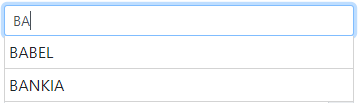
\includegraphics[width=10cm, keepaspectratio]{img/Autocomplete.PNG}
  \caption{Ejemplo de componente web Autocomplete.}\label{fig:component_autocomplete}
\end{figure}

Sus entradas son:

		\begin{itemize}
		\item \textbf{url:} URL de datos de referencia a la que consulta el componente, ver Subsección~\ref{subsec:reference_endpoints}.
		\item \textbf{placeholder:} Texto opcional que se muestra en la entrada de texto cuando el usuario no ha escrito nada.
		\item \textbf{footer:} Texto opcional que se muestra como pie de la entrada de texto.
		\item \textbf{value:} Variable que contiene el texto ingresado en la entrada de texto.
		\item \textbf{onChange:} Función de tipo callback que se ejecuta cuando hay cambios en la entrada de texto.
		\item \textbf{onSelect:} Función de tipo callback que se ejecuta cuando el usuario selecciona una sugerencia.
		\item \textbf{onSubmit:} Función de tipo callback que se ejecuta cuando el usuario presiona la tecla \emph{introducir}.
		\item \textbf{styleClasses:} Clases adicionales de estilos que se pueden añadir al componente.
		\end{itemize}

\subsubsection{AutocompleteMultiple}
\label{subsec:wc_autocomplete_multiple}
Este componente es una entrada de texto que ofrece al usuario una lista de sugerencias como ayuda para completar el texto que está ingresando,
similar al componente descrito anteriormente en la Subsubsección~\ref{subsec:wc_autocomplete}, pero que de forma diferente a este permite seleccionar múltiples valores que se muestran a continuación de la entrada de texto.
Los elementos aparecen filtrados según el texto que el usuario va escribiendo.
Para ofrecer la lista de sugerencias este formulario realiza una petición HTTP a uno de los puntos de API definidos en la Subsección~\ref{subsec:reference_endpoints}.
Este componente se muestra en la Figura~\ref{fig:component_autocomplete_multiple}

\begin{figure}
  \centering
  
\includegraphics[width=10cm, keepaspectratio]{img/AutocompleteMultiple.PNG}
  \caption{Ejemplo de componente web AutocompleteMultiple.}\label{fig:component_autocomplete_multiple}
\end{figure}

Sus entradas son:

		\begin{itemize}
		\item \textbf{url:} URL de datos de referencia a la que consulta el componente, ver Subsección~\ref{subsec:reference_endpoints}.
		\item \textbf{placeholder:} Texto opcional que se muestra en la entrada de texto cuando el usuario no ha escrito nada.
		\item \textbf{footer:} Texto opcional que se muestra como pie de la entrada de texto.
		\item \textbf{values:} Variable que contiene las lista de valores ingresados en la entrada de texto.
		\item \textbf{setValues:} Función que establece el valor de la variable \emph{values}.
		\item \textbf{styleClasses:} Clases adicionales de estilos que se pueden añadir al componente.
		\end{itemize}

\subsubsection{CardSkeleton}
\label{subsec:wc_card_skeleton}
Componente visual que muestra una tarjeta con datos en blanco, utilizado para mantener una experiencia de usuario agradable durante el tiempo que tardan en cargarse algunos que se consulta al API REST.
Este componente se muestra en la Figura~\ref{fig:component_card_skeleton}

\begin{figure}
  \centering
  
\includegraphics[width=15cm, keepaspectratio]{img/CardSkeleton.PNG}
  \caption{Ejemplo de componente web CardSkeleton.}\label{fig:component_card_skeleton}
\end{figure}

Sus entradas son:

		\begin{itemize}
		\item \textbf{lines:} Número de líneas en blanco que componen la tarjeta.
		\end{itemize}

\subsubsection{Checkbox}
\label{subsec:wc_checkbox}
Este componente permite seleccionar un valor booleano para una variable mediante un elemento de tipo casilla de verificación, o un interruptor dependiendo del estilo que se elija.
Este componente se muestra en la Figura~\ref{fig:component_checkbox}

\begin{figure}
  \centering
  
\includegraphics[width=3cm, keepaspectratio]{img/Checkbox.PNG}
  \caption{Ejemplos de componentes web Checkbox.}\label{fig:component_checkbox}
\end{figure}

Sus entradas son:

		\begin{itemize}
		\item \textbf{value:} Variable que contiene el valor de la casilla o interruptor.
		\item \textbf{setValue:} Función que establece el valor de la variable \emph{value} en los cambios de estado de la casilla o interruptor.
		\item \textbf{labelOff:} Texto que acompaña al elemento cuando está desmarcado.
		\item \textbf{labelOn:} Texto que acompaña al elemento cuando está marcado.
		\item \textbf{type:} Por defecto \emph{checkbox}, muestra una casilla de verificación si su valor es \emph{checkbox} o un interruptor si su valor es \emph{switch}.
		\item \textbf{disabled:} Si se estable su valor a \emph{true}, deshabilita el componente para que no sea modificable.
		\end{itemize}

\subsubsection{Chip}
\label{subsec:wc_chip}
Componente de tipo visual que permite representar un texto envuelto en un óvalo. Se usa para reprensentar un elemento en un listado de valores.
Este componente se muestra en la Figura~\ref{fig:component_chip}

\begin{figure}
  \centering
  
\includegraphics[width=12cm, keepaspectratio]{img/Chip.PNG}
  \caption{Ejemplo con varios componentes Chip seguidos.}\label{fig:component_chip}
\end{figure}

Sus entradas son:

		\begin{itemize}
		\item \textbf{value:} Texto del elemento de tipo \emph{Chip}.
		\end{itemize}

\subsubsection{ClosableChip}
\label{subsec:wc_closable_chip}
Componente de tipo visual que permite representar un texto envuelto en un óvalo, similar al componente Chip~\ref{subsec:wc_chip}, pero que a diferencia de este permite ser eliminado realizando click en un botón de aspa.
Se usa para reprensentar un elemento eliminable en un listado de valores.
Este componente se muestra en la Figura~\ref{fig:component_closable_chip}

\begin{figure}
  \centering
  
\includegraphics[width=11cm, keepaspectratio]{img/ClosableChip.PNG}
  \caption{Ejemplo con varios componentes ClosableChip seguidos.}\label{fig:component_closable_chip}
\end{figure}

Sus entradas son:

		\begin{itemize}
		\item \textbf{value:} Texto del elemento de tipo \emph{Chip}.
		\item \textbf{onClose:} Función que se ejecuta cuando se realiza click en el botón de aspa.
		\end{itemize}


\subsubsection{DateInput}
\label{subsec:wc_date_input}
Este componente es una entrada de texto que permite al usuario ingresar fechas.
Este componente se muestra en la Figura~\ref{fig:component_date_input}

\begin{figure}
  \centering
  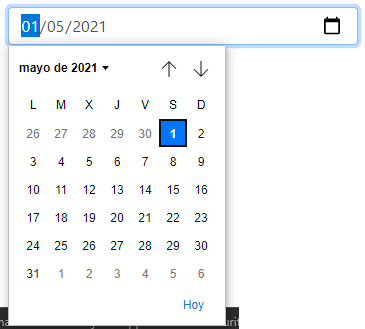
\includegraphics[width=7cm, keepaspectratio]{img/DateInput.PNG}
  \caption{Ejemplo de componente web DateInput.}\label{fig:component_date_input}
\end{figure}

Sus entradas son:

		\begin{itemize}
		\item \textbf{footer:} Texto opcional que se muestra como pie de la entrada de texto.
		\item \textbf{value:} Variable que contiene el texto ingresado en la entrada de texto.
		\item \textbf{onChange:} Función de tipo callback que se ejecuta cuando hay cambios en la entrada de texto.
		\item \textbf{disabled:} Si se establece a \emph{true}, la entrada de texto permanece deshabilitada para que no sea modificable.
		\item \textbf{styleClasses:} Clases adicionales de estilos que se pueden añadir al componente.
		\end{itemize}

\subsubsection{Modal}
\label{subsec:wc_modal}
Este componente web es una ventana modal que emerge en la página.
Se utiliza para destacar operaciones que requieren atención especial por parte del usuario en el contexto de una vista.
Este componente se muestra en la Figura~\ref{fig:component_modal}

\begin{figure}
  \centering
  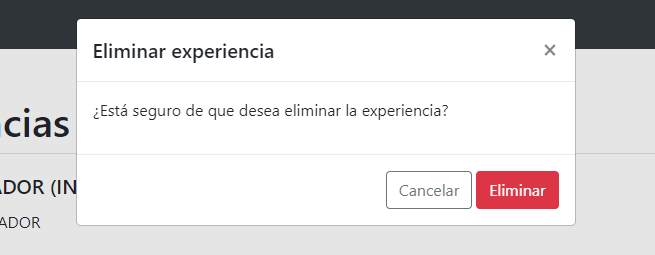
\includegraphics[width=10cm, keepaspectratio]{img/Modal.PNG}
  \caption{Ejemplo de componente web Modal.}\label{fig:component_modal}
\end{figure}

Sus entradas son:

		\begin{itemize}
		\item \textbf{title:} Título de modal.
		\item \textbf{children:} Una lista de dos elementos HTML (o componentes web) que el modal puede mostrar como contenido, el primero en el cuerpo del modal y el segundo en el pie del modal.
		\item \textbf{isShown:} Variable que controla si el modal se muestra o no.
		\item \textbf{close:} Función que maneja el cierre del modal.
		\item \textbf{additionalClasses:} Clases adicionales de estilos que se pueden añadir al componente.
		\end{itemize}

\subsubsection{MoneyInput}
\label{subsec:wc_money_input}
Este componente es una entrada de texto que permite al usuario ingresar cantidades de dinero.
Este componente se muestra en la Figura~\ref{fig:component_money_input}

\begin{figure}
  \centering
  
\includegraphics[width=7cm, keepaspectratio]{img/MoneyInput.PNG}
  \caption{Ejemplo de componente web MoneyInput.}\label{fig:component_money_input}
\end{figure}

Sus entradas son:

		\begin{itemize}
		\item \textbf{placeholder:} Texto opcional que se muestra en la entrada de texto cuando el usuario no ha escrito nada.
		\item \textbf{footer:} Texto opcional que se muestra como pie de la entrada de texto.
		\item \textbf{value:} Variable que contiene el dinero ingresado en la entrada de texto.
		\item \textbf{onChange:} Función de tipo callback que se ejecuzta cuando hay cambios en la entrada de texto.
		\item \textbf{currency:} Código ISO de la moneda en la cual se introduce la cantidad.
		\item \textbf{styleClasses:} Clases adicionales de estilos que se pueden añadir al componente.
		\end{itemize}

\subsubsection{NavbarUser}
\label{subsec:wc_navbar_user}
Este componentemuestra el usuario que está en sesión en la barra superior de navegación.
Además le permite cerrar sesión mediante un botón desplegable.
Este componente consulta directamente al punto de API de obtención de usuario para recuperar los datos del usuario en sesión. Ver~\ref{subsec:get_user}.
Este componente se muestra en la Figura~\ref{fig:component_navbar_user}

\begin{figure}
  \centering
  
\includegraphics[width=6cm, keepaspectratio]{img/NavbarUser.PNG}
  \caption{Ejemplo de componente web NavbarUser.}\label{fig:component_navbar_user}
\end{figure}

\subsubsection{NegotiableWorkExperience}
\label{subsec:wc_negotiable_work_experience}
Este componente de tipo tarjeta permite operar sobre los campos de una experiencia laboral, modificando la visibilidad de los campos de cara a realizar una oferta o solicitud de información.
Cada uno de los campos privados de la experiencia laboral posee su propio interruptor que controla la visibilidad, el usuario elije si quiere mantener un campo privado o ofrecerlo/pedirlo como público.
Este componente se muestra en la Figura~\ref{fig:component_negotiable_work_experience}

\begin{figure}
  \centering
  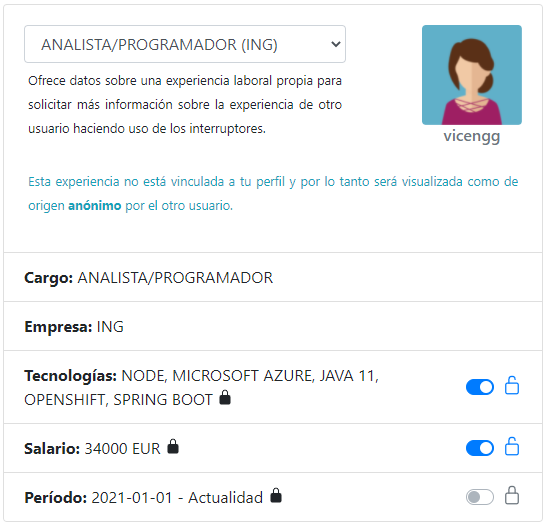
\includegraphics[width=10cm, keepaspectratio]{img/NegotiableWorkExperience.PNG}
  \caption{Ejemplo de componente web NegotiableWorkExperience.}\label{fig:component_negotiable_work_experience}
\end{figure}

Sus entradas son:

		\begin{itemize}
		\item \textbf{workExperience:} Objeto con el contenido de la experiencia laboral sobre la que se va a hacer el ofrecimiento/solicitud de visibilidad, ver definición de \emph{WorkExperienceEntity} en la Subsección~\ref{subsec:work_experience_entity}.
		\item \textbf{children:} Lista de tres elementos HTML. La tarjeta puede contener hasta tres elementos HTML (o componentes web) en su cuerpo. Los dos primeros representados a la izquierda del avatar del usuario y el último justo debajo.
		\item \textbf{visibilityRequest:} Variable que contiene la información de la visibilidad de la experiencia laboral que se está manipulando en el componente, ver definición de \emph{VisibilityRequest} en la Subsección~\ref{subsec:negotiation_value_objects}.
		\item \textbf{setVisibilityRequest:} Función que establece el valor de la variable \emph{visibilityRequest}.
		\item \textbf{disabled:} Si se establece a \emph{true} deshabilita el componente para evitar su modificación.
		\end{itemize}

\subsubsection{NegotiationSummary}
\label{subsec:wc_negotiation_summary}
Este componente de tipo tarjeta muestra de forma resumida el último estado de una negociación, es decir, si está pendiente, aceptada o cancelada, los datos que los usuarios ofrecen y solicitan y los usuarios que intervienen en ella.
Este componente se muestra en la Figura~\ref{fig:component_negotiation_summary}

\begin{figure}
  \centering
  
\includegraphics[width=15cm, keepaspectratio]{img/NegotiationSummary.PNG}
  \caption{Ejemplo de componente web NegotiationSummary.}\label{fig:component_negotiation_summary}
\end{figure}

Sus entradas son:

		\begin{itemize}
		\item \textbf{negotiation:} Objeto con el contenido de la negociación de la cual se está mostrando el resumen, ver definición de \emph{NegotiationEntity} en la Subsección~\ref{subsec:negotiation_entity}.
		\item \textbf{user:} Objeto que contiene la información del usuario en sesión, ver definición de \emph{User} en la Subsección~\ref{subsec:common_classes}.
		\end{itemize}


\subsubsection{OwnWorkExperience}
\label{subsec:wc_own_work_experience}
Este componente de tipo tarjeta muestra de forma resumida el contenido de una experiencia laboral del usuario en sesión, así como la visibilidad de los campos. Además permite al usuario eliminar su experiencia laboral y navegar a la vista de edición de experiencias laborales.
Este componente se muestra en la Figura~\ref{fig:component_own_work_experience}

\begin{figure}
  \centering
  
\includegraphics[width=15cm, keepaspectratio]{img/OwnWorkExperience.PNG}
  \caption{Ejemplo de componente web OwnWorkExperience.}\label{fig:component_own_work_experience}
\end{figure}

Sus entradas son:

		\begin{itemize}
		\item \textbf{workExperience:} Objeto con el contenido de la experiencia laboral de la que se muestran los datos, ver definición de \emph{WorkExperienceEntity} en la Subsección~\ref{subsec:work_experience_entity}.
		\item \textbf{afterDelete:} Función de tipo callback que se ejecuta después del borrado de la experiencia laboral.
		\item \textbf{editable:} Si se establece a \emph{true} permite eliminar y navegar a la vista de modifiación de la experiencia laboral.
		\end{itemize}


\subsubsection{Radio}
\label{subsec:wc_radio}
Este componente contiene una serie de botones de radio que permiten elegir entre varias opciones para establecer una variable.
Este componente se muestra en la Figura~\ref{fig:component_radio}

\begin{figure}
  \centering
  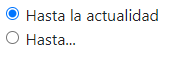
\includegraphics[width=5cm, keepaspectratio]{img/Radio.PNG}
  \caption{Ejemplo de componente web Radio.}\label{fig:component_radio}
\end{figure}

Sus entradas son:

		\begin{itemize}
		\item \textbf{options:} Un objeto de tipo JSON que alimenta de opciones al componente. Cada clave representa el identificador de una posible opción, mientras que cada valor representa el texto que se mostrará para esta opción por pantalla.
		\item \textbf{selected:} Variable que contiene la opción seleccionada.
		\item \textbf{changeOption:} Función de tipo callback que se ejecuta cuando la opción del componente cambia.
		\end{itemize}

\subsubsection{RequestButton}
\label{subsec:wc_request_button}
Este componente de tipo botón dispara peticiones HTTP cuando se hace click en él.
Este componente se muestra en la Figura~\ref{fig:component_request_button}

\begin{figure}
  \centering
  
\includegraphics[width=5cm, keepaspectratio]{img/RequestButton.PNG}
  \caption{Ejemplo de componente web RequestButton.}\label{fig:component_request_button}
\end{figure}

Sus entradas son:

		\begin{itemize}
		\item \textbf{text:} Texto del botón.
		\item \textbf{url:} URL a la que realizará las llamadas HTTP.
		\item \textbf{method:} Método HTTP, por defecto \emph{GET}.
		\item \textbf{body:} Cuerpo de la solicitud HTTP, por defecto vacío.
		\item \textbf{headers:} Cabeceras de la solicitud HTTP, por defecto incluye la cabecera \emph{Content-Type: application/json}.
		\item \textbf{styleClasses:} Clases de estilo adicionales que se le pueden añadir al botón.
		\item \textbf{onSucces:} Función de tipo callback que se ejecuta cuando la petición ha terminado y permite manejar la respuesta.
		\end{itemize}


\subsubsection{Select}
\label{subsec:wc_select}
Este componente genera un elemento de tipo seleccionable que permite elegir entre varias opciones en un menú desplegable.
Este componente se muestra en la Figura~\ref{fig:component_select}

\begin{figure}
  \centering
  
\includegraphics[width=10cm, keepaspectratio]{img/Select.PNG}
  \caption{Ejemplo de componente web Select.}\label{fig:component_select}
\end{figure}

Sus entradas son:

		\begin{itemize}
		\item \textbf{values:} Un objeto de tipo JSON que alimenta de opciones al componente. Cada clave representa el identificador de una posible opción, mientras que cada valor representa el texto que se mostrará en el desplegable para esa opción.
		\item \textbf{onChange:} Función de tipo callback que se ejecuta cuando hay cambios en el seleccionable.
		\item \textbf{styleClasses:} Clases adicionales de estilos que se pueden añadir al componente.
		\end{itemize}

\subsubsection{WorkExperience}
\label{subsec:wc_work_experience}
Este componente de tipo tarjeta muestra de forma resumida el contenido de una experiencia laboral resultado de una búsqueda.
Este componente se muestra en la Figura~\ref{fig:component_work_experience}

\begin{figure}
  \centering
  
\includegraphics[width=15cm, keepaspectratio]{img/WorkExperience.PNG}
  \caption{Ejemplo de componente web WorkExperience.}\label{fig:component_work_experience}
\end{figure}

Sus entradas son:

		\begin{itemize}
		\item \textbf{workExperience:} Objeto con el contenido de la experiencia laboral de la que se muestran los datos, ver definición de \emph{WorkExperienceEntity} en la Subsección~\ref{subsec:work_experience_entity}.
		\item \textbf{editable:} Si se establece a \emph{true} habilita un botón que permite navegar a la vista de negociación.
		\end{itemize}

\subsubsection{WorkExperienceSummary}
\label{subsec:wc_work_experience_summary}
Este componente de tipo tarjeta muestra de forma resumida el contenido de una experiencia laboral vinculada a una negociación en la vista de detalles de negociación.
Este componente se muestra en la Figura~\ref{fig:component_work_experience_summary}

\begin{figure}
  \centering
  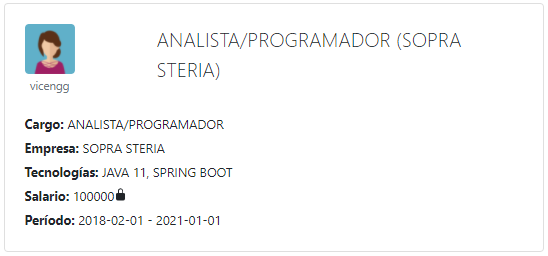
\includegraphics[width=10cm, keepaspectratio]{img/WorkExperienceSummary.PNG}
  \caption{Ejemplo de componente web WorkExperienceSummary.}\label{fig:component_work_experience_summary}
\end{figure}

Sus entradas son:

		\begin{itemize}
		\item \textbf{workExperience:} Objeto con el contenido de la experiencia laboral de la que se muestran los datos, ver definición de \emph{WorkExperienceEntity} en la Subsección~\ref{subsec:work_experience_entity}.
		\item 		\textbf{visibilityRequest:} Variable que contiene la información de la visibilidad de la experiencia laboral de la que se muestran los datos, ver definición de \emph{VisibilityRequest} en la Subsección~\ref{subsec:negotiation_value_objects}.
		\item \textbf{setVisibilityRequest:} Función que establece el valor de la variable \emph{visibilityRequest}.
		\end{itemize}









\section{Vistas}
\label{sec:views}
[TODO]

\section{Casos de uso}
\label{sec:use_cases}
[TODO]



%%%%%%%%%%%%%%%%%%%%%%%%%%%%%%%%%%%%%%%%%%%%%%%%%%%%%%%%%%%%%%%%%%%%%%%%%%%%%%%%
%%%%%%%%%%%%%%%%%%%%%%%%%%%%%%%%%%%%%%%%%%%%%%%%%%%%%%%%%%%%%%%%%%%%%%%%%%%%%%%%
% EXPERIMENTOS Y VALIDACIÓN %
%%%%%%%%%%%%%%%%%%%%%%%%%%%%%%%%%%%%%%%%%%%%%%%%%%%%%%%%%%%%%%%%%%%%%%%%%%%%%%%%

\cleardoublepage
\chapter{Experimentos y validación}

[TODO]


%%%%%%%%%%%%%%%%%%%%%%%%%%%%%%%%%%%%%%%%%%%%%%%%%%%%%%%%%%%%%%%%%%%%%%%%%%%%%%%%
%%%%%%%%%%%%%%%%%%%%%%%%%%%%%%%%%%%%%%%%%%%%%%%%%%%%%%%%%%%%%%%%%%%%%%%%%%%%%%%%
% RESULTADOS %
%%%%%%%%%%%%%%%%%%%%%%%%%%%%%%%%%%%%%%%%%%%%%%%%%%%%%%%%%%%%%%%%%%%%%%%%%%%%%%%%

\cleardoublepage
\chapter{Resultados}

[TODO]


%%%%%%%%%%%%%%%%%%%%%%%%%%%%%%%%%%%%%%%%%%%%%%%%%%%%%%%%%%%%%%%%%%%%%%%%%%%%%%%%
%%%%%%%%%%%%%%%%%%%%%%%%%%%%%%%%%%%%%%%%%%%%%%%%%%%%%%%%%%%%%%%%%%%%%%%%%%%%%%%%
% CONCLUSIONES %
%%%%%%%%%%%%%%%%%%%%%%%%%%%%%%%%%%%%%%%%%%%%%%%%%%%%%%%%%%%%%%%%%%%%%%%%%%%%%%%%

\cleardoublepage
\chapter{Conclusiones}
\label{chap:conclusiones}


\section{Consecución de objetivos}
\label{sec:consecucion-objetivos}

[TODO]

\section{Aplicación de lo aprendido}
\label{sec:aplicacion}

[TODO]

\section{Lecciones aprendidas}
\label{sec:lecciones_aprendidas}

[TODO]

\section{Trabajos futuros}
\label{sec:trabajos_futuros}

[TODO]


%%%%%%%%%%%%%%%%%%%%%%%%%%%%%%%%%%%%%%%%%%%%%%%%%%%%%%%%%%%%%%%%%%%%%%%%%%%%%%%%
%%%%%%%%%%%%%%%%%%%%%%%%%%%%%%%%%%%%%%%%%%%%%%%%%%%%%%%%%%%%%%%%%%%%%%%%%%%%%%%%
% APÉNDICE(S) %
%%%%%%%%%%%%%%%%%%%%%%%%%%%%%%%%%%%%%%%%%%%%%%%%%%%%%%%%%%%%%%%%%%%%%%%%%%%%%%%%

\cleardoublepage
\appendix
\chapter{Manual de usuario}
\label{app:manual}

[TODO]

%%%%%%%%%%%%%%%%%%%%%%%%%%%%%%%%%%%%%%%%%%%%%%%%%%%%%%%%%%%%%%%%%%%%%%%%%%%%%%%%
%%%%%%%%%%%%%%%%%%%%%%%%%%%%%%%%%%%%%%%%%%%%%%%%%%%%%%%%%%%%%%%%%%%%%%%%%%%%%%%%
% BIBLIOGRAFIA %
%%%%%%%%%%%%%%%%%%%%%%%%%%%%%%%%%%%%%%%%%%%%%%%%%%%%%%%%%%%%%%%%%%%%%%%%%%%%%%%%

\cleardoublepage

% Las siguientes dos instrucciones es todo lo que necesitas
% para incluir las citas en la memoria
\bibliographystyle{abbrv}
\bibliography{memoria}  % memoria.bib es el nombre del fichero que contiene
% las referencias bibliográficas. Abre ese fichero y mira el formato que tiene,
% que se conoce como BibTeX. Hay muchos sitios que exportan referencias en
% formato BibTeX. Prueba a buscar en http://scholar.google.com por referencias
% y verás que lo puedes hacer de manera sencilla.
% Más información:
% http://texblog.org/2014/04/22/using-google-scholar-to-download-bibtex-citations/

\end{document}
